\documentclass[12pt,a4paper,openright,twoside]{book}
\usepackage[utf8]{inputenc}
\usepackage{disi-thesis}
\usepackage{code-lstlistings}
\usepackage{notes}
\usepackage{shortcuts}
\usepackage{acronym}

\school{\unibo}
\programme{Corso di Laurea Magistrale in Ingegneria e Scienze Informatiche}
\title{Static Analysis of Aggregate Programs through Compiler Plugins}
\author{Francesco Magnani}
\date{\today}
\subject{Software Process Engineering}
\supervisor{Danilo Pianini}
\cosupervisor{Nicolas Farabegoli}
\morecosupervisor{Angela Cortecchia}
\session{III}
\academicyear{2023-2024}

% Definition of acronyms
\acrodef{IoT}{Internet of Thing}
\acrodef{vm}[VM]{Virtual Machine}
\acrodef{IDE}[IDE]{Integrated Development Environment}
\acrodef{CI}[CI]{Continuous Integration}
\acrodef{AST}[AST]{Abstract Syntax Tree}
\acrodef{KAPT}{Kotlin Annotation Processing Tool}
\acrodef{KSP}{Kotlin Symbol Processing}
\acrodef{IR}{Intermediate Representation}
\acrodef{DSL}{Domain Specific Language}
\acrodef{IR}{Intermediate Representation}
\acrodef{FIR}{Frontend Intermediate Representation}
\acrodef{PSI}{Programming Structure Interface}
\acrodef{TDD}{Test-Driven Development}


\mainlinespacing{1.241} % line spacing in mainmatter, comment to default (1)

\begin{document}

\frontmatter\frontispiece

\begin{abstract}	
Max 2000 characters, strict.
\end{abstract}

\begin{dedication} % this is optional
Optional. Max a few lines.
\end{dedication}

%----------------------------------------------------------------------------------------
\tableofcontents   
\listoffigures     % (optional) comment if empty
\lstlistoflistings % (optional) comment if empty
%----------------------------------------------------------------------------------------

\mainmatter

%----------------------------------------------------------------------------------------
\chapter{Introduction}
\label{chap:introduction}
%----------------------------------------------------------------------------------------

Analyzing characteristics of the source code without necessarily building and
executing it --- i.e., static analysis --- is a process that has been studied and
implemented in various forms during the last decades. Various tools have been
developed to perform such a task, each with its own strengths and weaknesses.
%
The need for such a tool is often evident in the software development process,
where ensuring the \textbf{quality} and \textbf{robustness} of software systems
is a critical concern. Using code quality analysis techniques is also a powerful
mean to avoid situations of ``technical debt''
\cite{DBLP:conf/sigsoft/ErnstBONG15}, that targets the system quality in
maintenance and evolution.

As the system grows in complexity, so does the variety of errors and
vulnerabilities that can be detected through tools (e.g., concurrency management
issues, error handling, etc.). At the same time, adhering to coding standards
helps to avoid both trivial and non-trivial errors from the outset.
Many tools exist to enforce these coding standards and to detect violations and,
moreover, these are usually among the easiest types of tools to integrate, often
already included within \acp{IDE}.
%
The effectiveness of static analysis tools has been the subject of various
studies,  \cite{DBLP:journals/jss/LenarduzziPSLP23} evaluating their detection
capabilities, agreement, and precision. Some of these studies revealed a low
degree of agreement among the tools and highlighted the need for a better
understanding of their actual capabilities. More advance tools have been used
also to rewrite code and help with the development of very complex systems,
like \emph{Coccinelle} for the Linux kernel
\cite{DBLP:conf/eurosys/PadioleauLHM08}\cite{DBLP:conf/usenix/LawallM18}.
%
More over, in the last years, the static analysis tools have become more popular
and easier to use, becoming protagonists of many \ac{CI} pipelines
\cite{DBLP:conf/msr/ZampettiSOCP17} that automatically performs checks on the
entire source code, embracing change and evolution of the software without
making it a threat \cite{DBLP:books/daglib/0015650}, backed by a solid safety
net. 

\section{Static Analysis for novel paradigms}

Despite all this, these tools are not always available out-of-the-box,
especially in the case of new and experimental language paradigms. Developing
useful static analysis tools means having a \textbf{deep understanding of the
language} used to write the code, as well as \textbf{knowing the paradigm well
enough} in order to reason about the main pitfalls and points of failure present
within it.
%
Beyond this, static analysis tools are inherently difficult to develop, as they
must be exceptionally reliable and robust. They serve as critical foundations
for software development, and they are among the last places where one would
want to encounter a bug. Any flaw in these tools can lead to incorrect analysis,
misguiding developers and potentially introducing severe issues into a codebase.
%
Moreover, from a technical standpoint, developing such tools also requires
building a substantial integration layer with other systems to ensure their
usability. For instance, they need to seamlessly integrate with \acp{IDE}, code
editors, and development pipelines, further increasing the complexity of their
implementation.

Even considering all of this, the challenge of developing these tools extends
beyond technical complexity. For a static analysis tool to be created, the
programming paradigm in question must first reach a sufficient level of
\textbf{interest} and \textbf{usability} within the software development
landscape: only then does the need for such a tool become evident. However, the
growth and adoption of a new paradigm are often inhibited by the very absence of
these tools, which have become essential in most development contexts. This
creates a self-perpetuating cycle: without adequate tooling, a paradigm
struggles to gain traction, yet without widespread adoption, there is little
incentive to develop the necessary tools.
%
As a result, developers and industry stakeholders tend to fall back on
well-established tools with mature and certified ecosystems, reinforcing the
dominance of existing paradigms. This, in turn, leads to significant
\emph{technical debt}, as developers are forced to work within paradigms that
may not be the most suitable for the problem at hand. Beyond that, this
situation also causes many promising research projects to remain confined within
academia, preventing their potential impact on the broader software development
industry. 

It is clear now that knowing how can this cycle be broken is a key point in 
the development of new paradigms and tools.

\section{The role of Domain Specific Languages} \label{sec:dsls}

When implementing a new paradigm in the form of a programming language,
\acp{DSL} are often used. A \ac{DSL} is a specialized language designed for a
specific domain, rather than a general-purpose programming language. Since many
new paradigms do not require extensive general-purpose functionality, \acp{DSL}
often provide a natural and efficient way to express the paradigm’s core
concepts.
%
One of the key advantages of \acp{DSL} is their ability to bring the target
domain closer to its usage and manipulation. This often results in a syntax that
is more intuitive, sometimes even resembling natural language, and encourages a
more declarative way of writing code. Additionally, because \acp{DSL} are
inherently more restricted in scope than general-purpose languages, developing
static analysis tools for them tends to be significantly easier. Their limited
expressiveness reduces the complexity of the analysis, making it more feasible
to create robust and effective tooling. 

Recently, many new \acp{DSL} have been implemented as \emph{internal} to a host
language. Internal \acp{DSL} are embedded within a general-purpose language,
using the host language's syntax and semantics to define the domain-specific
constructs. This approach offers several advantages, including the ability to
leverage the host language's ecosystem and tooling, without having to develop a
compiler from scratch and manage all the necessary checks. 
%
Additionally, internal \ac{DSL} users can use already existing libraries
available for the host language to make their life easier. This approach,
however, also comes with its disadvantages, the main one being the limitations
in their expressiveness, as the host language's capabilities can
\textbf{constrain syntax and semantics}. For this reason, developing internal
\acp{DSL} could suffer from scalability issues when the lack of full control
over the language becomes an obstacle to the paradigm reflection in the code.
Moreover, implementing custom static checks over the code could be difficult
when the host language does not provide the necessary hooks to do so (i.e., 
meta-programming capabilities).

In conclusion, even though internal \acp{DSL} can be a solution to the first
half of the problem --- i.e., the adoption and implementation of the paradigm
with less technical challenges --- they still suffer from the lack of proper
tooling for specific static analysis.

\section{Enabling static analysis through Compiler Plugins}

If looked from another perspective, automated static analysis tools and
compilers share significant similarities in their operations. Both perform
thorough examinations of source code without executing it, aiming to identify
errors, enforce coding standards, and optimize performance. Most of what
compilers do on the static analysis side is to facilitate code optimization and
error detection during the compilation process. In fact, a compiler can be
viewed as a form of static analysis tool, as it analyzes code to generate
executable programs and associated debugging information
\cite{DBLP:journals/queue/Thomson21}.
%
Specialized static analysis tools, on the other hand, extend beyond the
capabilities of standard compilers by offering additional functionalities and
broader diagnostic capabilities. They offer a broader range of diagnostic rules,
enabling the detection of specific and uncommon bugs that compilers might
overlook.
%
What if, however, the compiler were extended beyond its core functionality,
incorporating specialized capabilities that go beyond the scope of a
general-purpose environment? These extensions could be designed to address the
unique requirements of a specific project or domain. This is precisely where
\textbf{compiler plugins} come into play.

Compiler plugins are dynamic modules that interact with the compiler during its
various phases, enabling the introduction of new functionalities or the
modification of existing behaviors. They serve as intermediaries that can
inspect, modify, or enhance the compilation process, providing developers with
the flexibility to implement domain-specific checks, optimizations, or
transformations, all without altering the compiler's core architecture. 
%
For instance, in the context of the GNU Compiler Collection
(GCC), plugins allow for the addition of new features without necessitating
modifications to the compiler itself (mostly, again, for optimization purposes).

\subsection{Types of Compiler Plugins}

Compiler plugins can be broadly categorized based on the phase of compilation they target:

\begin{itemize}
  \item \textbf{Frontend Plugins}: These plugins operate during the initial
  stages of compilation, focusing on tasks such as syntax analysis, semantic
  analysis, and \ac{IR} generation (i.e., an internal data structure used by the
  compiler). They are useful also for implementing custom syntax extensions,
  enforcing coding standards, or performing static code analyzes. For example,
  in the \emph{Rust} programming language, compiler plugins can introduce new
  syntax extensions and lint checks. 

  \item \textbf{Backend Plugins}: Functioning in the latter stages of
  compilation, backend plugins are concerned with code optimization, machine
  code generation, and platform-specific adjustments. They can be utilized to
  implement custom optimizations, support additional hardware
  architectures and more.
\end{itemize}

\subsubsection{Compiler Plugins in Kotlin}

Kotlin, a statically typed programming language developed by JetBrains, offers
robust support for compiler plugins, allowing developers to highly customize the
compilation process to their specific needs. 
%
Kotlin's compiler architecture facilitates the creation of plugins that can
modify or extend its behavior during compilation. For example, the
\emph{all-open} compiler plugin in Kotlin allows classes annotated with a
specific annotation to be open without the explicit \lstinline{open} keyword,
adapting Kotlin to the requirements of frameworks that need classes to be
open. 

When guiding developers towards the creation of compiler plugins, JetBrains
compares them to \textbf{Annotation Processors}
\cite{JetBrains:KotlinCompilerPlugin}. Annotation processors are a powerful
feature in many modern programming languages, including Java and Kotlin, that
allow developers to generate code, validate code, and perform various
compile-time checks based on \textbf{annotations} present in the source code.
%
In Java, annotation processors are part of the Java Compiler API and can be used
to generate additional source files, validate the correctness of the code, and
even modify the \ac{AST} of the code being compiled. They are
commonly used in frameworks and libraries to reduce boilerplate code and enforce
coding standards.
%
Kotlin also supports annotation processors through the \ac{KAPT} --- which is, in
fact, a compiler plugin itself --- that allows Kotlin code to interoperate with
Java annotation processors and, more recently, the \ac{KSP}, another compiler
plugin introduced as ``an API that you can use to develop lightweight compiler
plugins''. The former enables developers to leverage existing Java annotation
processors in their Kotlin projects and the latter, on the other hand, provides
a more efficient and Kotlin-specific way to generate code at compile time,
offering a new approach that is much more integrated with Kotlin symbols.

\subsection{Advantages of Compiler Plugins}

Compiler plugins and Annotation Processors, however, have some very distinct
functionalities. While Annotation Processors are limited to generating source
code and performing checks based on annotations, compiler plugins can exploit a
very powerful API that can create and modify byte-code, elements inside the
\ac{IR} and more, allowing the developers to solve a whole new class of
meta-programming problems. In addition, the use of annotations in the code could
make it more ``cluttered'' from the perspective of a DSL, reducing it to
constructs that belong more strictly to the host language, while the compiler
plugin would not need these annotations. Of course, Annotation Processors are
typically easier to write and maintain than compiler plugins, but this extra
cost can be worth in several cases, for example in the scenario that will be
presented in this thesis.

\subsection{Main challenges and requirements}

At the time of writing, the development of frontend compiler plugins in Kotlin is
still a relatively less explored area compared to the backend ones. Because of the 
very little documentation and examples available, the development of frontend 
compiler plugins can be a challenging task, that quite often requires inspecting 
the Kotlin compiler source code to understand how to interact with it.
%
Frontend compiler plugins can be implemented using \textit{Extensions} to the
Kotlin compiler, a topic that will be covered more in detail in the following
chapters. This thesis presents the development process of a frontend compiler
plugin designed to build upon an existing \textit{backend} plugin. The primary
purpose of this frontend plugin is to perform static checks on source code,
ensuring compliance with specific rules related to the functionality of the
pre-existing backend plugin. To better understand the target rules developed
within this frontend plugin and its context, it is necessary to first introduce 
the backend plugin and the project it is part of.

\paragraph{Structure of the Thesis}

This thesis follows the development process of a frontend compiler plugin from
its initial steps, addressing the key challenges encountered as well as the
solutions proposed during the research and implementation phases. The next
chapter, \cref{chap:background}, provides an overview of the ongoing project for
which this frontend plugin is being developed, alongside the technical
background necessary to understand how a plugin can interact with the Kotlin
compiler.
%
\Cref{chap:contribution} delves into the core development process of the plugin,
discussing the design decisions, alternative approaches considered, and the
final implementation of the proposed \textbf{checkers}. Subsequently,
\cref{chap:evaluation} evaluates the plugin’s behavior, with a particular focus
on the testing methodology adopted, including the integration of a custom
testing framework named \emph{Subjekt}, developed specifically for this purpose.
%
Lastly, \cref{chap:conclusion} summarizes the primary contributions of this
thesis and outlines potential directions for future work, building on the
results and insights gained throughout this research.

%----------------------------------------------------------------------------------------
\chapter{Background: the Collektive case}
\label{chap:background}
%----------------------------------------------------------------------------------------

As already stated, the development of the frontend compiler plugin presented in
this thesis will be built on top of an existing backend plugin. The backend
plugin is part of a larger project named \emph{Collektive}, a Kotlin
multiplatform framework that provides a \ac{DSL} for the \textbf{Aggregate
Computing} \cite{Beal2015} paradigm. This chapter will provide an overview of
the concepts behind Collektive as well as the feature behind its backend plugin
and Kotlin compiler plugins development in general.

\section{Aggregate Computing: a novel paradigm}

The Aggregate computing paradigm is a novel approach to ``design, create and
maintain'' \cite{Beal2015} complex distributed systems, particularly in the 
context of the Internet of Things (IoT). The paradigm shifts the focus from
individual devices to regions of devices, abstracting away the details of their
number, position, and behavior. This abstraction enables developers to reason
about distributed systems in terms of \emph{collective} operations over spatial and
temporal fields, rather than device-to-device interactions. 

The foundation of aggregate programming is built on \textbf{field calculus}
\cite{Beal2014TowardsAU}, a set of constructs designed for \emph{spatial
computing}. These constructs enable the implementation of robust coordination
mechanisms, such as self-stabilizing and scalable operations \cite{Viroli2018}
\cite{DBLP:journals/jlap/ViroliBDACP19}, which adapt dynamically to changes in
the environment. Applications of aggregate programming are particularly
impactful in large-scale scenarios, such as crowd management during public
events, where distributed devices coordinate to provide services like crowd
density estimation, dispersal advice, and navigation support.

Aggregate computing formalism has been proposed in various ways, introducing
syntaxes and semantics to support distributed, collective behaviors in dynamic
systems. Field calculus, as a foundational model, supports aggregate computing
by enabling global-level manipulation of computational fields through a
minimalistic syntax. 
%
Tools like Protelis \cite{DBLP:conf/saso/PianiniBV17}, ScaFi
\cite{DBLP:conf/ecoop/CasadeiV16} and the recently proposed eXchange Calculus
(XC) \cite{DBLP:journals/jss/AudritoCDSV24} extend field calculus principles,
providing programming frameworks and language constructs to bridge the gap
between theoretical models and practical implementations.

Managing the programming line of action for these kinds of systems is not
trivial, but several approaches have already been proposed, including static and
dynamic checks that can spot subtle bugs and vulnerabilities in the code, by
focusing on concepts like \textbf{neighborhood interactions} and \textbf{domain
alignment} \cite{DBLP:conf/saso/AudritoDVC16}.

\subsection{Applications and critical aspects}

In Aggregate Computing, the main model of the system consists of a \emph{network of 
intercommunicating devices}, which can be \emph{close} to one another therefore 
introducing a concept of \textbf{neighborhood}. 
%
Each device is equipped with sensors and actuators, enabling interaction with an
environment, and can communicate with other devices through a
\emph{message-passing} system. 

A key aspect of Aggregate Computing regards the execution model, which is based
on a local program identical for all devices. The system is governed by a
continuously executed loop that makes the devices \emph{receive messages},
\emph{produce a result through their internal behavior} and finally \emph{send
values to neighbors}. 
%
This simple structure allows for system to show self-organizing behaviors
emerging from the \emph{collective} of devices, and contemplates even complex
interactions of the devices with the environment (e.g. creation of new devices).

Finally, as already said, the \emph{field calculus} model can be implemented
through an ad-hoc API and syntax to perform operations on a \emph{computational
field} (i.e., a mapping from device locations to values in our example)
manipulating it over time, defining interactions between devices and finally
creating the emergent behavior.
%
After the previous tools already cited, it is now necessary to
introduce the Aggregate Computing framework that will be the target of the
frontend plugin in this thesis: \emph{Collektive}.

\section{Collektive: an Aggregate Computing framework}

\emph{Collektive} is a modern Aggregate Computing framework developed in Kotlin 
that allows developers to easily write Aggregate Computing programs through a 
flexible \emph{internal} DSL. The framework is designed to be multiplatform,
targeting both JVM and JavaScript platforms, as well as native ones. 
%
Compared to some other existing Aggregate Computing frameworks, Collektive
offers a modern and idiomatic approach to writing Aggregate Computing programs,
with a static type system (as it is internal to Kotlin) and few, expressive
constructs like \lstinline{neighboring} and \lstinline{exchange}, which can be
used to implement a broad variety of interactions between devices (and also
Aggregate Computing patterns).

The project is organized in modules, with the main one being the \lstinline{dsl}
and \lstinline{compiler-plugin}, and is tested using the Alchemist simulator
\cite{DBLP:journals/jos/PianiniMV13}. 

\subsection{Collektive DSL: main concepts} \label{sec:collektive-dsl}

In order to understand how to work on Collektive programs, we first need to
understand its main usage. Collektive DSL is centered around the
\lstinline{aggregate} function, which is the entry point for the Aggregate
Computing program. The function uses a local ID to identify the device on which
is executed on and then accepts a function type with receiver
\lstinline{compute: Aggregate<ID>.() -> R} that performs the aggregate
computation using the \lstinline{Aggregate} interface members.
%
The \lstinline{Aggregate} interface provides several functions that represent
the main constructs of Collektive's implementation of the Aggregate Computing
paradigm. The most important ones are:
\begin{itemize}
  \item \lstinline{neighboring}: a function that observes expressions on
  neighbors, returning the related field;
  \item \lstinline{exchange}: a function that, taken from the documentation of
  Collektive, ``manages the computation of values between neighbors in a
  specific context''. In practice, it can be used to compute a new field of 
  values starting from initial values of neighbors;
  \item \lstinline{evolve}: updates an initial value iteratively computing an
  expression at each device;
  \item \lstinline{share}: performs a field computation starting from neighbors'
  values, reducing them to a single value and then sharing it with neighbors. 
  It can be used to actuate a ``space-time evolution'' on the field.
\end{itemize}

Some of these constructs is present also in a variant that allows to return a
different type of value from the initial one; the name of the variant is 
the same of the original function but with the suffix \lstinline{-ing} (e.g., 
\lstinline{exchanging}, \lstinline{evolving} etc.).

Just by using these four constructs, already complex collective behaviors can
be achieved. Besides that, the Collektive DSL hides several operations through
the already mentioned compiler plugin. 

\subsection{Collektive Compiler Plugin}

As previously introduced, Collektive provides an already integrated
\textbf{backend compiler plugin}. This plugin is responsible for managing the
\emph{alignment of aggregate computation}, a very important concept when dealing
with Aggregate computing programs, faced in several studies
\cite{DBLP:conf/forte/DamianiVPB15} \cite{DBLP:conf/saso/AudritoDVC16}.
%
Essentially, the domain alignment is a necessary step to ensure that when a
device computes a value that depends on neighboring devices (e.g., through the
\lstinline{neighboring} construct, which retrieves values from neighbors), those
neighboring devices have computed the same expression in the same evaluation
round. This guarantees that shared computations remain consistent across
devices: it's necessary in order to \textbf{maintain consistency between field
values} and \text{prevent information leakage} because ``without it, information
may leak unexpectedly between devices that are evaluating different functions,
or may be “blocked” from passing between devices evaluating the same function''
\cite{DBLP:conf/forte/DamianiVPB15}.

Collektive \emph{backend} compiler plugins works by analyzing call sites and
function definitions in the code, intercepting the ones that involve aggregate
computation and that should, therefore, be ``aligned''. Essentially, this is
done by looking at \lstinline{Aggregate} interface usage in functions,
especially when used as receiver, and visiting their declarations, wrapping
aggregate constructs usages with special \lstinline{align} and
\lstinline{dealign} functions that perform domain alignment under the hood.
%
As we will see, this is not always automatic or safe in certain situations 
(e.g., loops), and the frontend extension will take care of these extra 
checks. 

But how do Kotlin compiler plugins work in general? Before diving into the 
core development of the frontend plugin, it is necessary to understand their
main structure and how they interact with the Kotlin compiler.

\section{Kotlin Compiler Plugins: general structure} 

Since Kotlin is a multiplatform language, the same source code can be compiled
into low-level code specific to different targets, such as the JVM, JavaScript,
and native platforms. In order to work with different targets, the Kotlin
compiler architecture is divided into two sub-parts: the \emph{frontend} and the
\emph{backend}\footnote{The following explanation is greatly
inspired from the work of \cite{moskala2023}, which provides a more
comprehensive overview of the Kotlin compiler plugins architecture.}.
%
The frontend is independent of the target, and for this reason its output can be 
reused when targeting different platforms. Currently, this part of the compiler 
is being migrated to the new K2 version, which is supposed to be much more 
efficient than the previous K1 version.
%
The backend, on the other hand, is mostly specific to the target platform, and
uses the output of the frontend to generate the final code. In reality, the
backends for JVM, JS, Native, and WASM share some parts: that will be analyzed
later. The general structure is summarized in
\cref{fig:kotlin-compiler-architecture}.

\begin{figure}
  \centering
  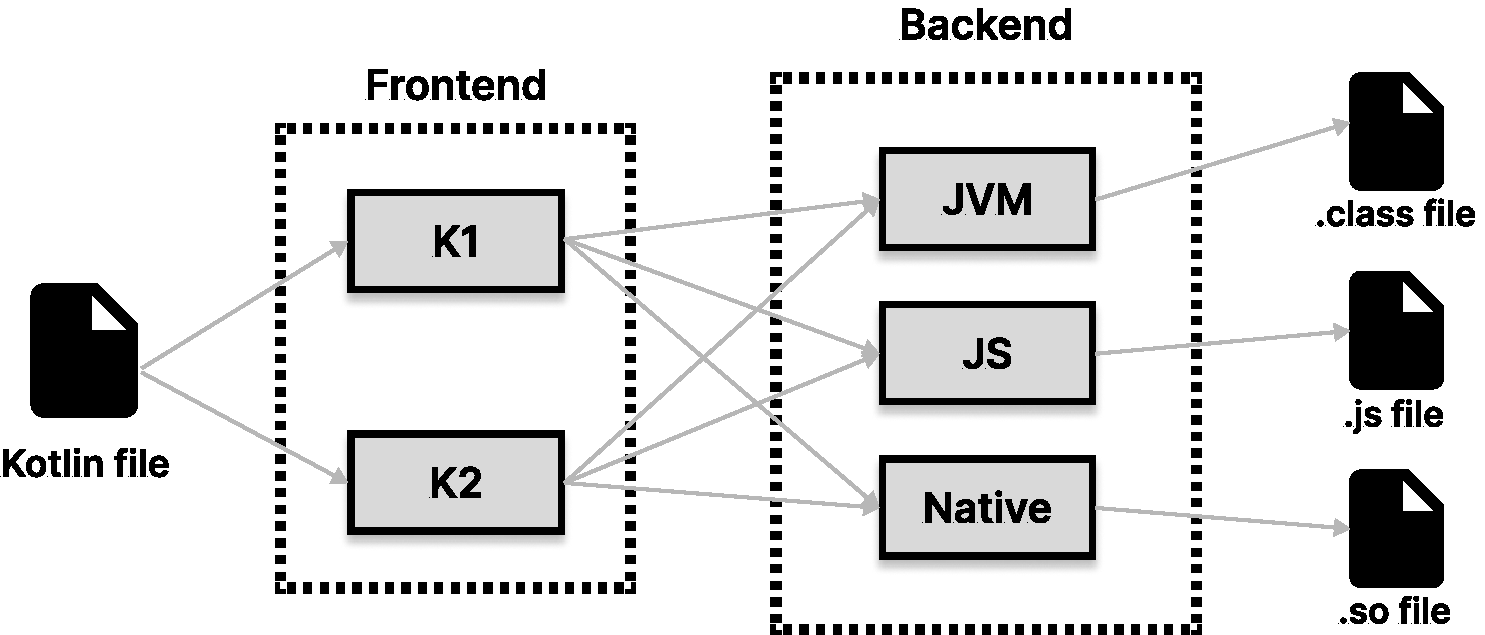
\includegraphics[width=.8\linewidth]{figures/kotlin-compiler-architecture.pdf}
  \caption{Kotlin compiler architecture. Adapted from the one at \cite{moskala2023}}
  \label{fig:kotlin-compiler-architecture}
\end{figure}

\subsection{Kotlin K2 and frontend plugins}

The frontend's output is not only used by the backend for the final one, but it
is also responsible for communicating with \acp{IDE} and build tools, providing
APIs to present errors, warnings, code completions and so on. 
%
To make this architecture modular, the Kotlin compiler provides a set of 
\acp{IR}, that the various steps of the workflow
can use to process the preceding steps' output. Both the frontend and the
backend creates this data structure, although they are very different. The 
backend's one is created starting from the output \ac{IR} of the frontend,
while the frontend's one is created from the Kotlin source code. 
The general workflow is summarized in \cref{fig:kotlin-compiler-workflow}.

\begin{figure}
  \centering
  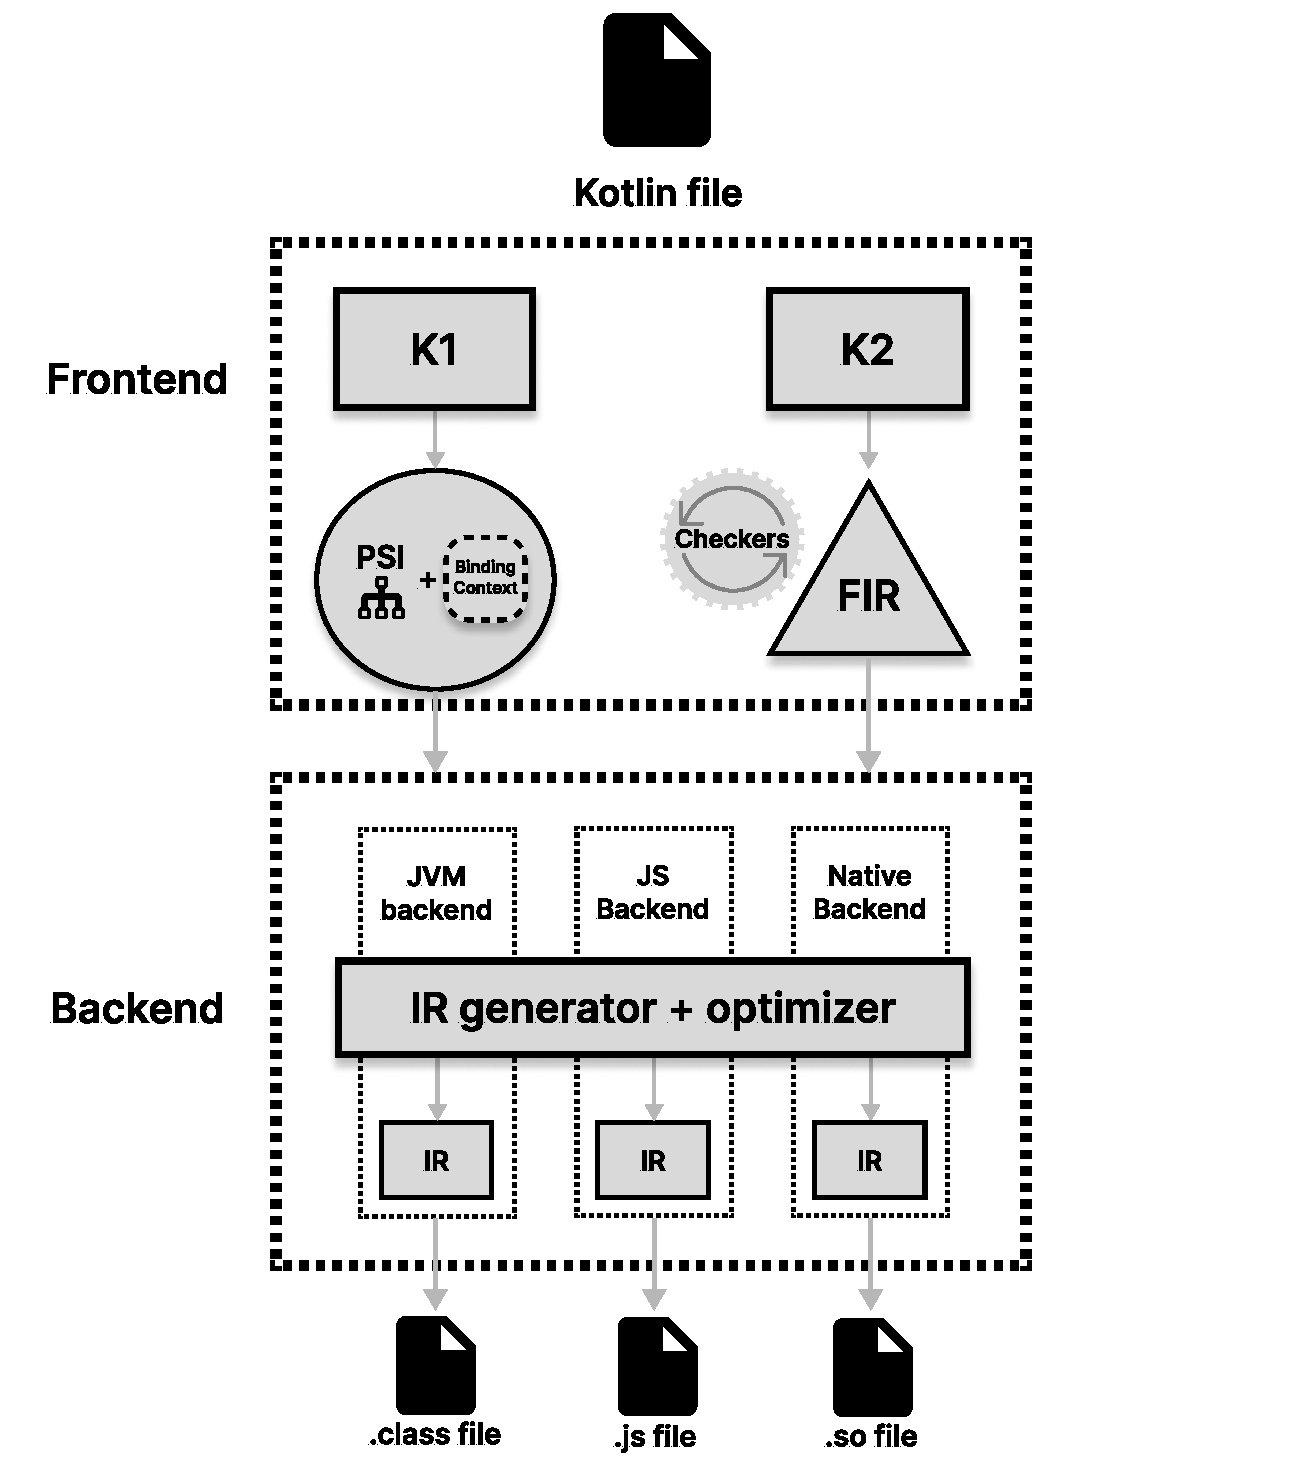
\includegraphics[width=.9\linewidth]{figures/kotlin-compiler-workflow.pdf}
  \caption{Kotlin compiler general workflow. Adapted and extended from the one
  at \cite{moskala2023}}
  \label{fig:kotlin-compiler-workflow}
\end{figure}

Before the so-called K2 frontend the compiler's frontend worked by
building the \ac{PSI}, a syntactic model of the parsed source code, and the
\lstinline{BindingContext}, that holds semantic information such as types and
symbol bindings (represented in \cref{fig:kotlin-compiler-workflow} as a whole). 
%
The new K2 frontend, on the other hand, builds the \ac{FIR}, a more powerful and
complete representation of Kotlin parsed code, capable of offloading some of the
work that was previously done by the backend and enabling powerful optimizations
and caching mechanisms. The raw \ac{PSI} is still being produced, but it is now
transformed into the \emph{raw FIR}, which again transforms in different stages,
filling the tree with semantic information. Finally, the resolved tree is passed
to the backend, which takes care of the platform-specific (backend) \ac{IR}, used
to generate the final code.

As we can see in \cref{fig:kotlin-compiler-workflow}, there is still another
process that hasn't been mentioned yet: the \emph{checkers}. During their stage
of execution, the checkers can inspect the \ac{FIR} and reports different
diagnostics. If some of them is considered ``critical'', in the sense that the
compilation should not proceed (e.g., a type error), the compilation is stopped,
and the backend is not executed: otherwise, the final \ac{IR} is passed to it.
%
The role of the checkers is particularly important in the context of this
thesis, and the way it's possible to interact with them is by means of
\textbf{extensions}.

\subsection{Extension mechanism}

Kotlin compiler extensions are mechanisms that allow developers to modify
various phases of the compilation process, either by analyzing and transforming
code at the \ac{FIR} level or by modifying the backend \ac{IR}. These extensions
enable advanced features such as additional type checks, automated code
generation, and optimizations, empowering Kotlin’s extensibility.
%
Like with compiler stages, extensions can be either frontend or backend as well.
While frontend extensions impact code analysis, syntax resolution, and IDE
support, backend extensions act right after the \emph{IR generation +
optimization} phase seen in \cref{fig:kotlin-compiler-workflow}. This
distinction makes frontend extensions more suitable for language-level changes
and linting rules, whereas backend extensions are primarily used for performance
optimizations and bytecode transformations.

K2 introduces multiple frontend extensions, all following the
\lstinline{Fir[Name]Extension} convention. In relation to what was previously
discussed, the \lstinline{FirAdditionalCheckersExtension} is particularly
important in this context, since it's a frontend extension that allows
developers to register \emph{additional checkers} to run during compilation.
These checkers can enforce custom coding rules, report warnings, or even prevent
compilation by issuing errors. More over, errors and warnings generated by this
extension appear in IDEs like IntelliJ IDEA, improving real-time code feedback.
This extension is used by Kotlin plugins like \emph{Kotlin Serialization},
which ensures that serialization-related constraints are properly followed, and
\emph{Arrow Meta}, which enforces functional programming best practices.

The extension mechanism is also used in the backend, where backend plugins can
intervene, but the extension that needs to be used in only one:
\lstinline{IrGenerationExtension}. This extension is invoked after the \ac{FIR}
phase has completed and the \ac{IR} has been generated. It allows modifications
to the IR tree before it is used for bytecode generation. Because IR sits
between the frontend and the platform-specific backend, changes made here can
impact the generated machine code without altering the high-level source
representation --- and, for this reason, it does not influence code analysis
in \acp{IDE} like IntelliJ IDEA. This extension is widely used in performance-critical
applications. For instance, \emph{Jetpack Compose} leverages it to transform
composable functions into an optimized internal representation. Similarly,
\emph{Kotlin Serialization} uses it to generate serialization methods dynamically,
ensuring they are both efficient and lightweight. However, modifying IR directly
can introduce breaking changes if not handled carefully. Since IR
transformations occur at a low level, even minor alterations can lead to
unintended consequences, making this extension a powerful but complex tool.

\subsubsection{IR generation inside Collektive} \label{sec:ir-generation-collektive}

Collektive backend plugin uses the \lstinline{IrGenerationExtension} to perform 
the operations we already discussed. To register an extension, the developer needs
to declare a class that extends \lstinline{CompilerPluginRegistrar}. Inside that,
the developer can register the extension using the \lstinline{registerExtension}
method that depends on the type of extension that is being registered. 
%
The core login of the plugin is then implemented in the extension itself. In the
case of the Collektive backend plugin, the class structure is summarized 
in \cref{fig:extensions-class-diagram}.

\begin{figure}
  \centering
  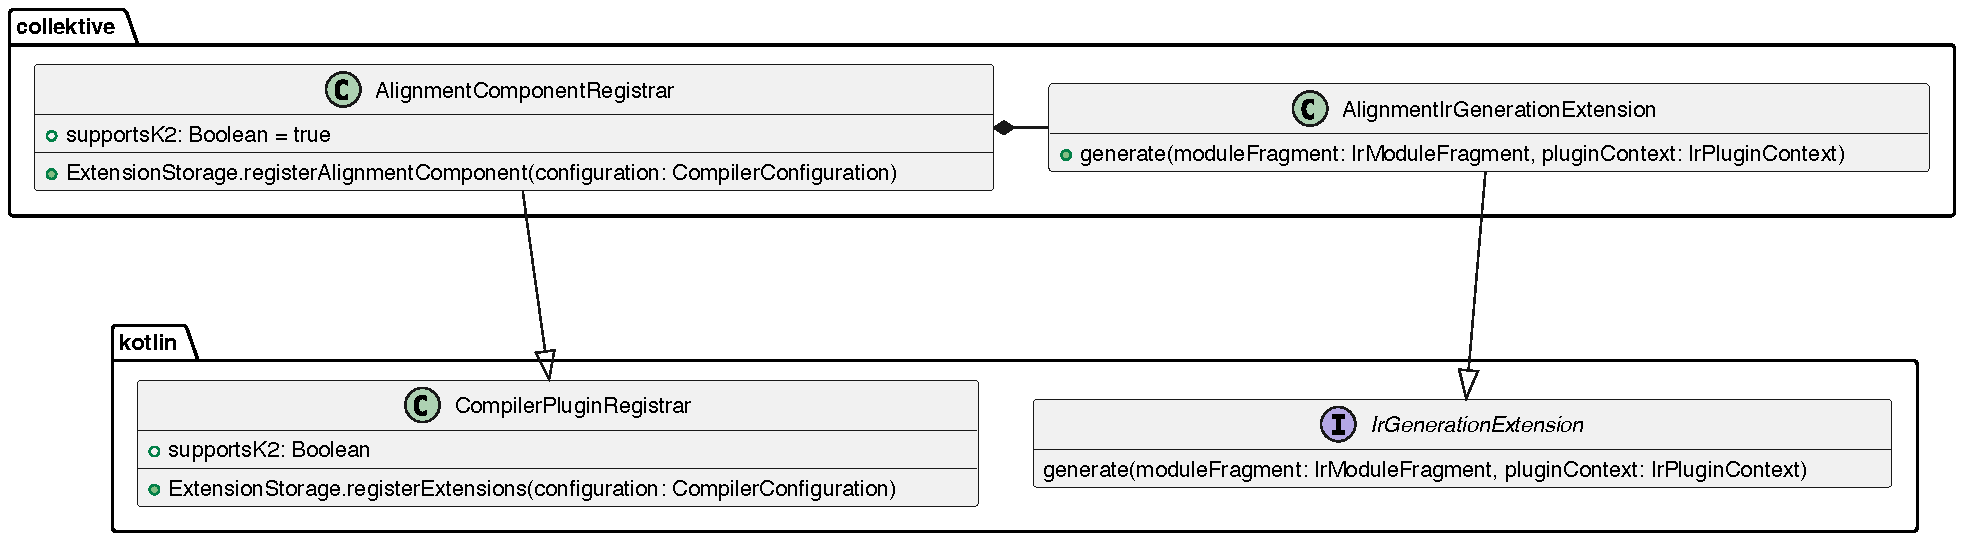
\includegraphics[width=.9\linewidth]{figures/extensions-class-diagram.pdf}
  \caption{Class diagram representing the top-level structure of the Collektive 
  backend compiler plugin. Note: the frontend plugin is not included yet.}
  \label{fig:extensions-class-diagram}
\end{figure}

Finally, to include the plugin, a \lstinline{META-INF/services} file is needed,
where the fully qualified name of the \lstinline{AlignmentComponentRegistrar} is
written, and the plugin is wrapped in a Gradle plugin that can be applied to the
project build. After the application of the frontend plugin also, the structure
of the project's components will be the one described in
\cref{fig:collektive-components-diagram}.

\begin{figure}
  \centering
  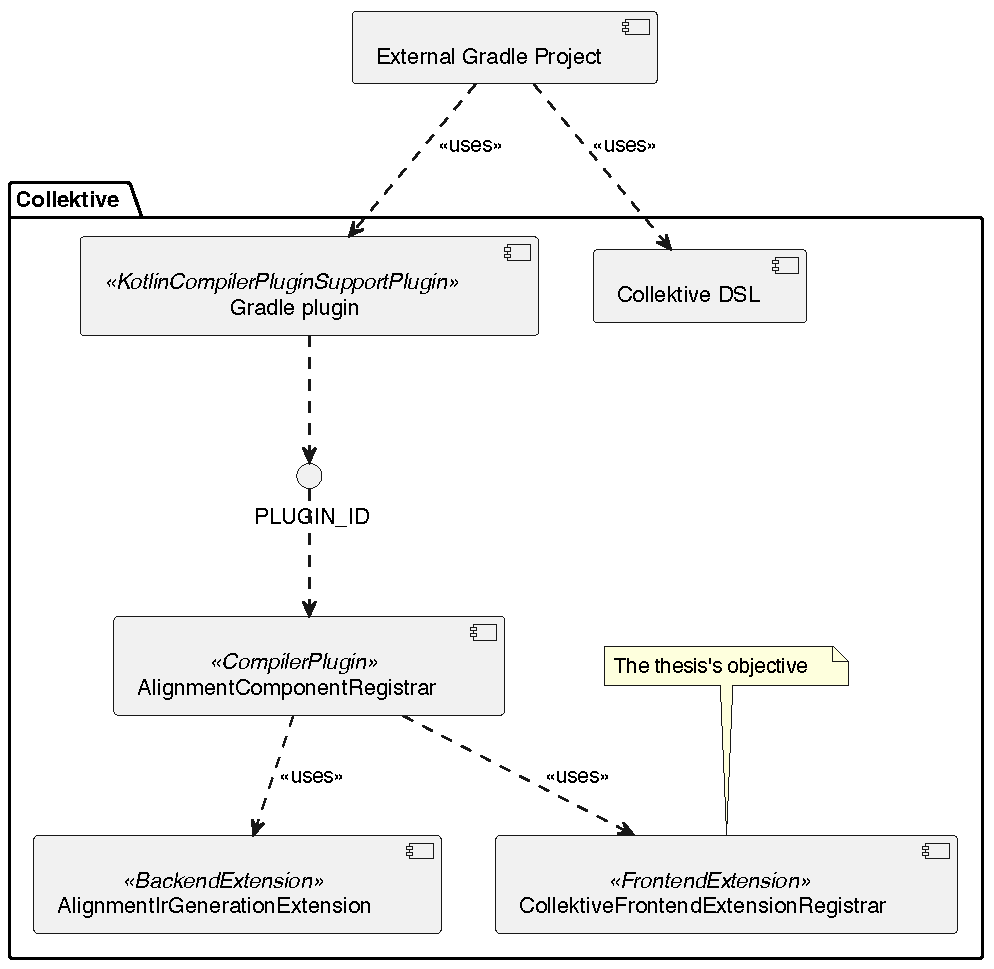
\includegraphics[width=.6\linewidth]{figures/collektive-components.pdf}
  \caption{Components of the Collektive project after the application of the frontend plugin}
  \label{fig:collektive-components-diagram}
\end{figure}

\section{DSL and Compiler Plugins}

In relation to what stated in \cref{sec:dsls}, the feature that is missing in
most \emph{internal} DSLs is the ability to perform static analysis on the code
that is written, and this is particularly difficult since the developers
struggle to intervene in the compilation process of the host language.
%
Compiler plugins seem perfect for this task since, in the case of Kotlin
compiler plugins at least, they can greatly influence the compilation process on
the frontend side and take care of the static analysis of the code. Collektive
is in fact internal to Kotlin and its main pitfalls --- and the ones of
Aggregate Computing in general --- which are currently not captured can be
spotted by a frontend plugin made for the job. 

In other words, the frontend plugin can take care of the ``other half of the 
problem'' introduced in \cref{sec:dsls}.

\subsection{The importance of Build Tools}

Considering all of this, it is important to mention the role of build tools in
the development process of a compiler plugin. Without a seamless integration of
the compiler plugin during the compilation process (and, as it will be shown,
the testing process as well), the development of a compiler plugin would be
cumbersome and error-prone. 
%
Needless to say, a well-configured build tool is a fundamental requirement in
this context. Within the Kotlin ecosystem --- on which this work focuses --- the
most widely used build tool is \emph{Gradle}, and it will serve as the
foundation for the implementations discussed in this thesis.

\subsection{Main motivations}

Before diving into the development of the frontend plugin, let's briefly
summarize the motivations behind the project. As previously mentioned, Aggregate
computing is still a relatively new paradigm, and some studies
\cite{DBLP:conf/saso/AudritoDVC16} already pointed out subtle bugs that can
occur when using some of its possible implementations. 
%
Collektive is not an exception and, in this particular case, developing a
frontend compiler plugin is motivated by three main reasons:
\begin{enumerate}
  \item \textbf{The backend plugin}: since a backend plugin is already present
  and necessary for the correct functioning of the framework, the frontend
  plugin can be simply built on top of it, extending its functionalities and
  ensuring that the user's operations are safe and within the scope of
  Collektive DSL correct usage principles.

  \item \textbf{The presence of an internal DSL}: when building a DSL, a
  developer must choose to make it \emph{internal} to a host language, like
  Kotlin, or \emph{external}, like Protelis \cite{DBLP:conf/saso/PianiniBV17},
  and so take care of the parsing and the compilation process in general.
  %
  As already said, internal \acp{DSL} are typically easier to use and to
  develop, but they can also be less flexible and more error-prone, because the
  developer does not have full control over the parsing process and therefore
  cannot always enforce the constraints that the DSL should have. This is the
  case with Collektive, and the frontend plugin can help in this regard.
  
  \item \textbf{The integration with the other development tools}: developing a
  frontend plugin integrates very well with the other tools that are already 
  used in most projects, for example:

  \begin{itemize}
    \item \textbf{IDE}: since the IntelliJ IDEA \ac{IDE} is the most indicated
    for Kotlin development and it has a very good support for the Kotlin
    compiler, the frontend plugin can leverage this support to provide real-time
    feedback for diagnostics and errors it produces, without the need of
    developing specific \ac{IDE} plugins.

    \item \textbf{Build tools}: the Gradle plugin that is used to apply the
    compiler plugin is pretty simple and needs almost zero modifications when
    extending the compiler plugin, differently from what would happen in the
    case of Gradle plugins wrapping external tools (e.g. \emph{ktlint}). This
    means that it can be easily maintained and integrated into other Gradle
    projects with low effort.

    \item \textbf{Rest of the pipeline}: the frontend plugin can be developed 
    very closely to the rest of the Collektive framework through submodules,
    adding dependencies between subprojects in a very clean and maintainable
    way.
  \end{itemize}
\end{enumerate}

Considering these motivations, we can now proceed with the actual development in
the next chapter.

%----------------------------------------------------------------------------------------
\chapter{Frontend plugin development}
\label{chap:contribution}
%----------------------------------------------------------------------------------------

In this chapter we will present the development process that lead to the creation of 
the frontend plugin inside the Collektive project.

\paragraph{Structure of this chapter}

In this chapter, we will first present the general workflow of the plugin's
checkers, then we will proceed presenting several \textbf{patterns} that were
detected observing the Collektive DSL codebase. These patterns represent bad or
inappropriate use cases of the Collektive DSL that are \textbf{not} captured by 
default. 
%
The way these patterns will be presented does not follow the chronological order 
of their development, but rather an order with an increasing level of complexity.
For this purpose, the patterns will be categorized into four main groups, 
reflecting the design decisions that were taken to approach the related problems,
highlighting the pros and cons of each approach. 

\textbf{Note}: the features of the Kotlin compiler explained and shown in
this chapter are \emph{experimental}, and therefore subject to possible instability
and frequent changes. The code snippets and examples provided are based on the
current state of the Kotlin compiler at the time of writing. 

\section{Adopted workflow}

After defining the \lstinline{CollektiveFrontendExtensionRegistrar} class that
wraps the frontend plugin, already introduce in \cref{sec:ir-generation-collektive}, the
first step is to register the actual extensions to the compiler using the
\lstinline{configurePlugin} method. For this plugin, the extension that will
be used is the already cited \lstinline{FirAdditionalCheckersExtension}, which
allows to register additional checkers to run during compilation.
%
This extension can contain an arbitrary number of checkers, each of them
assigned to different elements of the \ac{FIR} tree (e.g., expressions,
declarations etc.). All the checkers that will be presented are added 
through this extension. The final class structure is summarized in
\cref{fig:frontend-class-diagram}.

\begin{figure}
  \centering
  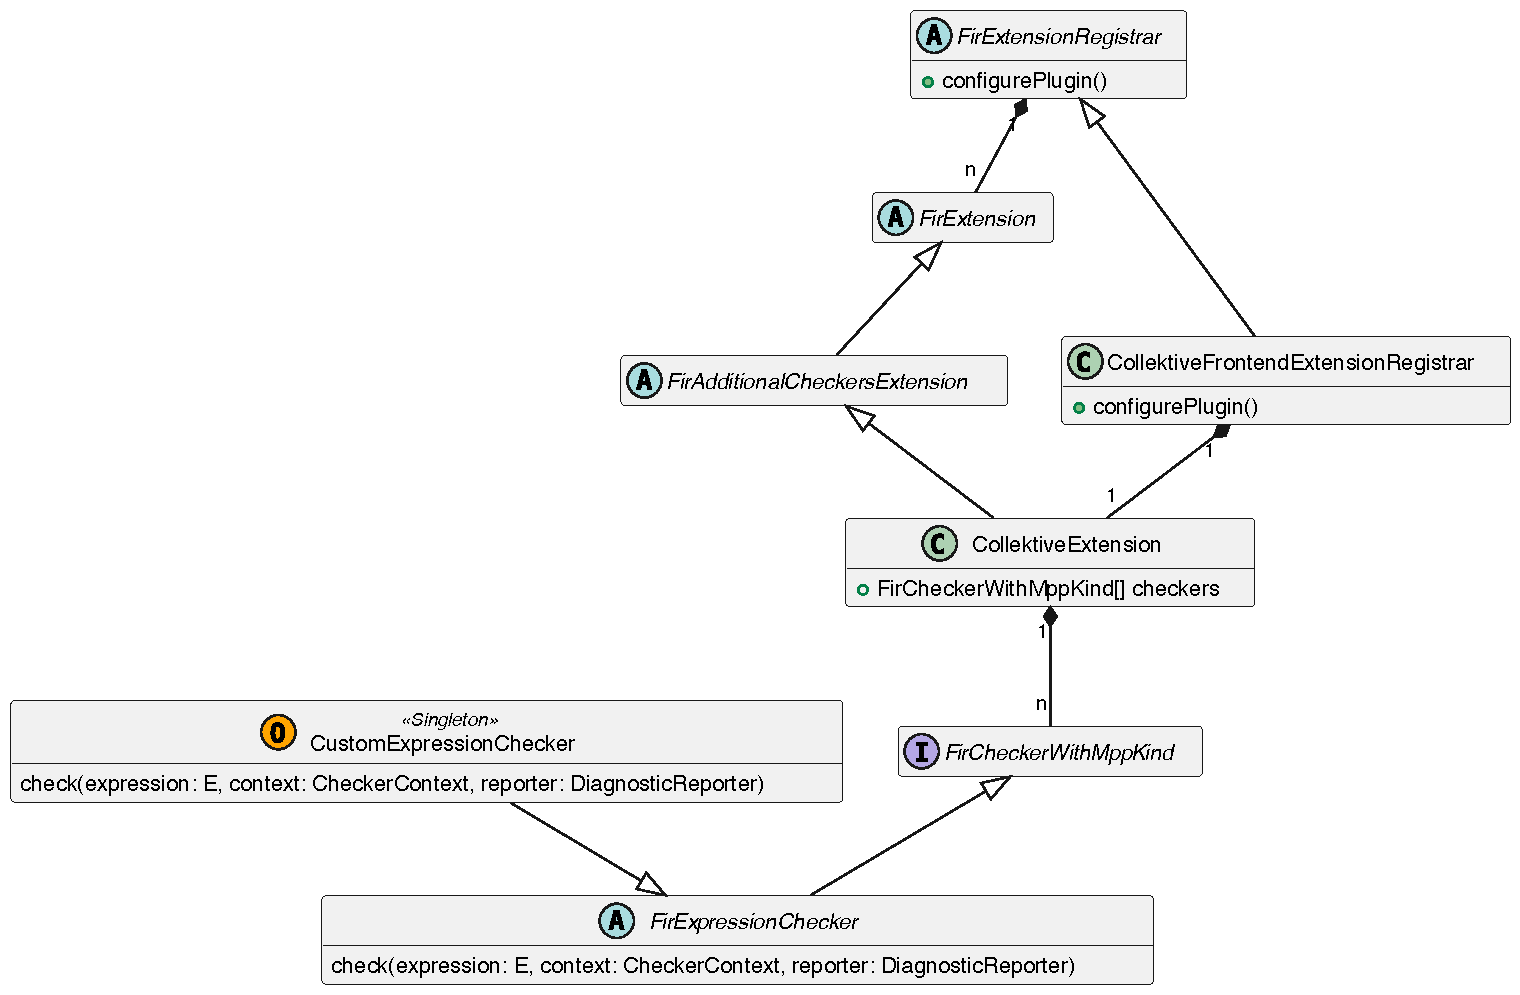
\includegraphics[width=.8\linewidth]{figures/frontend-class-diagram.pdf}
  \caption{Class diagram summarizing the structure of the frontend plugin}
  \label{fig:frontend-class-diagram}
\end{figure}

From this point on, the workflow of the plugin development will be as follows:

\begin{enumerate}
  \item \textbf{Pattern detection}: when a new pattern that needs to be captured
  by the plugin is detected, several examples of Collektive programs expecting a
  positive or negative  diagnostic are written (i.e., respectively, cases in
  which the diagnostic should be reported and cases where it shouldn't).
  \item \textbf{Test arrangement}: the examples previously written are used to 
  create a test suite that will be used as certification of the pattern's correct
  capture., following a \ac{TDD} approach.
  \item \textbf{Checker creation and implementation}: a new checker is created and
  added to the frontend extension, implementing the logic that will detect and 
  correctly report positives of the pattern's usages.
  \item \textbf{Adjustments and identification of corner cases (optional)}: during
  the checker's development some corner cases may arise that need to be handled 
  by this checker and added as regression tests. In this case, after the corner 
  cases are correctly identified, this goes back to step 2, working on the already
  created checker.
\end{enumerate}

In this chapter we will present these steps for each pattern except for the step
2, that will be covered in \cref{chap:evaluation}. 

\textbf{Note}: the code snippets that will be presented in the following
sections, if not appropriately specified in the code, present portions of code
that are \textbf{inside an Aggregate block}, therefore contained either in a
function that has the \lstinline{Aggregate} interface as receiver or in a 
\lstinline{aggregate} entry point block, since these are the places where 
the Collektive DSL can be used to specify aggregate behaviors. This has been
done for the sake of brevity and clarity.

\section{1st approach: direct Kotlin API usage}

The API that Kotlin provides to interact with the \ac{FIR} is sufficiently
powerful to be used to perform a wide range of operations and checks. The
first approach to the development of the checkers was to use this API directly,
without the need of any additional constructs or classes. This approach is the
most direct and simple, but it was used only for the simplest pattern, without a
very complex logic behind it.

\subsection{Pattern 1: explicit align/dealign}

One of the first pattern detected was the explicit usage of the
\lstinline{align} and \lstinline{dealign} functions of the Collektive DSL. These
functions are not supposed to be used directly by the developer because they are
already managed by the backend plugin, and their direct usage can lead to
inconsistent behavior and unexpected results. For how the Collektive DSL is
structured, it was not possible to prevent the usage of these functions directly
through the API, so the frontend plugin was put in charge of this task.

\subsubsection{Formal description}

Given two functions \lstinline{align} and \lstinline{dealign} available in the
\lstinline{Aggregate} interface, the pattern is satisfied when any of these
functions are used explicitly in the code. \Cref{lst:p1-example} shows an
example of this pattern.

\lstinputlisting[
  float, 
  language=Kotlin, 
  label={lst:p1-example},
  caption={Example of Pattern 1 detection in code}
]{listings/P1Example.kt}

\subsubsection{Design and Implementation}

One of the type of checkers available among \ac{FIR} checkers is the
\lstinline{FirFunctionCallChecker}, which is just a type alias for a
\lstinline{FirExpressionChecker} --- that is, a checker that takes care of
expressions in the code --- typed with a \lstinline{FirFunctionCall} --- i.e.,
an element of the \ac{FIR} tree representing a function call in the code. This
type of checker can inspect function calls usages, calling the \lstinline{check}
method of the checker with a \lstinline{FirFunctionCall} as parameter. 
%
To performs checks on the function call, we can inspect the properties of this
parameter. In this case we simply need to \textbf{compare the fully qualified
name} of the function with the one of the interested functions.

Getting the fully qualified name of the function is not directly supported by
the \ac{FIR} API, but it is possible to build a simple utility function that
retrieves it. The final implementation of the checker is shown in
\cref{lst:p1-checker}: some portions of the code are omitted for brevity.

\lstinputlisting[
  float, 
  language=Kotlin, 
  label={lst:p1-checker},
  caption={Implementation of the Pattern 1 checker: \lstinline{ExplicitAlignDealign}}
]{listings/P1Checker.kt}

The \lstinline{context} object is an instance of \lstinline{CheckerContext} and is 
used to provide contextual information to the checker.

The \lstinline{reportOn} method of the \lstinline{reporter} object is used to
report a diagnostic when the pattern gets detected. The parameter passed to this
method determine where the diagnostic is gonna be reported (i.e., the position
in the code) and the message shown to the user (in these checkers, specified
inside an object called \lstinline{FirCollektiveErrors}).

\section{2nd approach: declarative and modular API}

Even though the API available in the checker is flexible and already powerful,
it can be quite verbose if we need to implement utilities even for simple
operations like obtaining the fully qualified name of a function. To simplify
the development of the checkers and make them more modular, a small API was
developed to make declarative checks on the \ac{FIR} tree. This API is composed
of a set of functions with receiver that can be used to perform common
operations on the \ac{FIR} elements, for example to check if a Checker context
is \textbf{inside an Aggregate function or block}. Some of these utilities are
shown in \cref{lst:simple-api}.

\lstinputlisting[
  float, 
  language=Kotlin, 
  label={lst:simple-api},
  caption={Some utility functions of the simple API developed}
]{listings/SimpleApi.kt}

As we can see, we can perform checks on the \ac{FIR} tree using built-in methods
like \lstinline{containingElements}: we can use this method to check if a
\lstinline{FirElement} is contained inside a function that has a \emph{receiver
parameter} of a certain type, in this case the \lstinline{Aggregate} type, by
inspecting the name of the \emph{Class-like Symbol} (i.e., the symbol referred
to a class or similar entities like interfaces) to which it is related. 
%
Encapsulating this not really trivial operations in functions makes them still
reusable and declarative in the context of domain-specific checkers like the
ones we are developing. This greatly empowers the Kotlin \ac{FIR} API, making it
more interesting also for more complex cases that will be presented later.

\subsection{Pattern 2: simple aggregate operations in loops} \label{sec:p2}

The second pattern that was inspected is the usage of \emph{aggregate operations
inside loops}. This pattern is more complex because it reflects cases that are
not always inappropriate usages, but if not properly handled can lead to
problems during the alignment phase. 
%
When an aggregate construct (i.e., a function call that needs alignment between
devices) is called inside a loop (e.g. a \lstinline{for} loop), the alignment of
the computation fails because multiple devices are not able to align to the same
``instance'' of the call between the iterations. 
%
However, the alignment can succeed if the loop contains a \emph{custom alignment
operation}, that can be done using the \lstinline{alignedOn} method, which is
available inside the \lstinline{Aggregate} interface. This method accepts an
anonymous function that will be the subject of the alignment. 
%
Again, this behavior cannot be captured through the internal DSL alone, so the
frontend plugin is needed to handle this case. 

It could seem that this pattern is not overly complex to detect compared to the
previous one, but in reality just adding one more simple constraint makes the
range of possible cases that can be captured following this pattern much broader
and more varied. Consider the cases presented in \cref{lst:p2-corner-case}. 
\lstinputlisting[
  float, 
  language=Kotlin, 
  label={lst:p2-corner-case},
  caption={Corner case related to Pattern 2, where the construct is used inside 
  a nested function}
]{listings/P2CornerCase.kt}
These corner cases are exceptions to the general rule that we previously stated,
in fact:
\begin{itemize}
  \item In the first case, although, technically, the construct is ``present''
  inside the loop, it is not directly called by the loop itself, but by a nested
  function. Note that even though this can be seen as a corner case, this is
  valid Kotlin code and might appear, maybe as slightly modified versions of
  this one, in real use cases.
  \item In the second case, we have the required \lstinline{alignedOn} operation
  wrapping the Aggregate function call, but it is placed outside the loop,
  making the alignment operation useless.
  \item In the third case, the loop is done without alignment, but this is in
  fact correct because the construct is not iterated by the loop since a new
  aggregate instance is created at each iteration. This makes each of them
  like a separate Aggregate program, and the alignment is not necessary.
\end{itemize}

Many more cases regarding this pattern can be found, but some of these will be
presented as another, separated pattern in \cref{sec:p5}. For now, we will deal
with the simpler cases, described in the following, more formal description.

\subsubsection{Formal description}

Given a construct that loops through various iterations (e.g., a \lstinline{for}
statement, an anonymous function called when cycling collection elements like
\lstinline{map}, \lstinline{forEach} etc.) \emph{inside} an ``aggregate'' block,
the pattern is satisfied when an aggregate construct is used under one of the
following conditions:
\begin{enumerate}
  \item The construct is called inside this loop without a wrapping
  \lstinline{alignedOn} operation \emph{inside the loop} as well;
  \item The construct is called inside this loop as part of a static declaration
  (e.g., a nested function) whose use is not iterated by the loop.
\end{enumerate}

\subsubsection{Design and Implementation}

The description might still seem incomplete or vague to some extent, and the
reason is that some potential cases are still not captured. For now, though, the
developed checker will be able to capture the most common cases, and the rest,
as we will see, will be easily integrated when covering the Pattern 5. 

One possible way to approach this pattern is reasoning in terms of
\textbf{containing blocks}: starting from the aggregate function called, we
could be able to determine if the pattern is detected or not just by looking at
the \textbf{sorted list of containing blocks of the function call}. Starting
from there, we first inspect if a loop is, in fact, containing the function
call, and if so, we check for other elements like the presence of the
\lstinline{alignedOn} in the correct order. This procedure is summarized in
\cref{fig:p2-flowchart}.

\begin{figure}
  \centering
  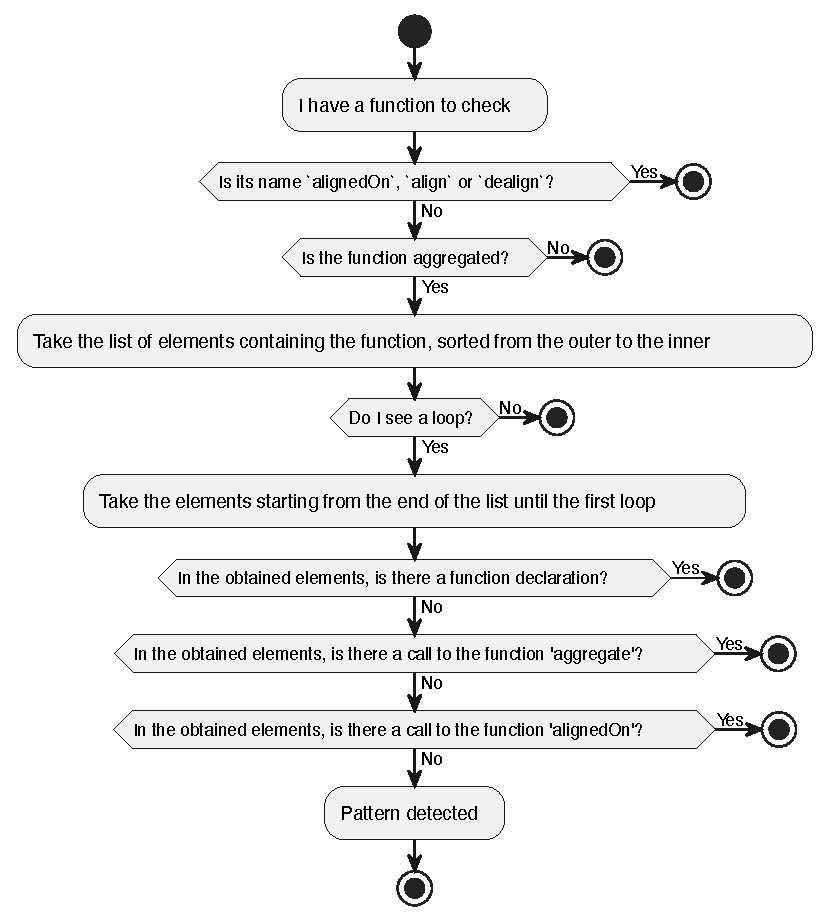
\includegraphics[width=.6\linewidth]{figures/p2-flowchart.pdf}
  \caption{Flowchart representing the procedure to detect Pattern 2}
  \label{fig:p2-flowchart}
\end{figure}

As we can see from the flowchart, the procedure ends immediately if the function
name is one of \lstinline{alignedOn}, \lstinline{align} or \lstinline{dealign},
since these are functions that do not require alignment. Thanks to Kotlin 
nullability system, we can perform these subsequent checks in a declarative way,
adding utilities to the simple API that we previously introduced and making it 
more extensible for more checks like this.
%
We first add these simple functions shown in \cref{lst:p2-api} to the API, and
then we can finally implement the checker, as shown in \cref{lst:p2-checker}. 

\lstinputlisting[
  float, 
  language=Kotlin, 
  label={lst:p2-api},
  caption={Utility functions added to help in the detection of Pattern 2}
]{listings/P2SimpleApi.kt}

\lstinputlisting[
  float, 
  language=Kotlin, 
  label={lst:p2-checker},
  caption={Implementation of the Pattern 2 checker: \lstinline{NoAlignInsideLoop}}
]{listings/P2Checker.kt}

As we can already see, implementing a checker with this approach has several
advantages: the code is readable and modular, and the logic is
declarative and easier to understand. This approach is also extensible and
can be easily adapted to other patterns that require similar checks.
%
This is, however, a very particular case that can be caught simply by looking at
containing elements. Once the pattern becomes more complex, adding concepts like
\emph{symbol's usage references} or \emph{structured operations with particular
requirements}, like nested anonymous calls or simply subsequent statements that
appear in the code that need to be checked together, this approach quickly
becomes less effective and more verbose, as it requires a very effective and
carefully designed API that cover as many cases as possible. 
%
It becomes quite clear that covering corner cases and patterns that reflect many
possible \ac{FIR} trees needs an approach that is more suitable to this kind of
data structures.

\section{3rd approach: visitor pattern}

One of the main design patterns that can be used to traverse a tree-like data 
structure is the \emph{visitor pattern}. This pattern is particularly useful 
when the tree structure is complex and the operations that need to be performed
on it are varied and not easily encapsulated in a single class.
%
The visitor pattern well fits the context of the Kotlin \ac{FIR}, since the
structure resembles the one of the \ac{AST} built by the Kotlin parser. 
Visitors are naturally used during the compilation process even if we don't
explicitly define any, since the compiler itself needs to traverse the tree to
perform the various operations that are needed to compile the code.
%
Moreover, Kotlin provides a set of utilities that can be used to implement
Visitors that fit the developer needs and that can be easily integrated into the
checkers in order to explore the \ac{FIR} structure behind the
\lstinline{FirElements} that are passed to the checkers.

Kotlin \ac{FIR} visitors are automatically generated inside the Kotlin compiler 
code in order to have a specific method for each type of \lstinline{FirElement}
that can be used to visit that element. All that is left to the developer is to
choose which type of visitor to extend in order to implement their own:

\begin{itemize}
  \item \lstinline{FirVisitor<R, D>}: a visitor where each visit method accepts
a \lstinline{D} parameter that can be used to pass data between the visit calls,
and a return type \lstinline{R} that can be used to return a result from the 
visitor.
  \item \lstinline{FirVisitorVoid}: a visitor where each visit method accepts
only the element to visit and returns nothing. Under the hood is simply a 
\lstinline{FirVisitor<Unit, Nothing?>}.
\end{itemize}

Depending on the specific task assigned to the visitor, the developer will
choose one of these two types of visitors and extend it into a new class. Their
structure is summarized in the class diagram of
\cref{fig:fir-visitors-class-diagram}.

\begin{figure}
  \centering
  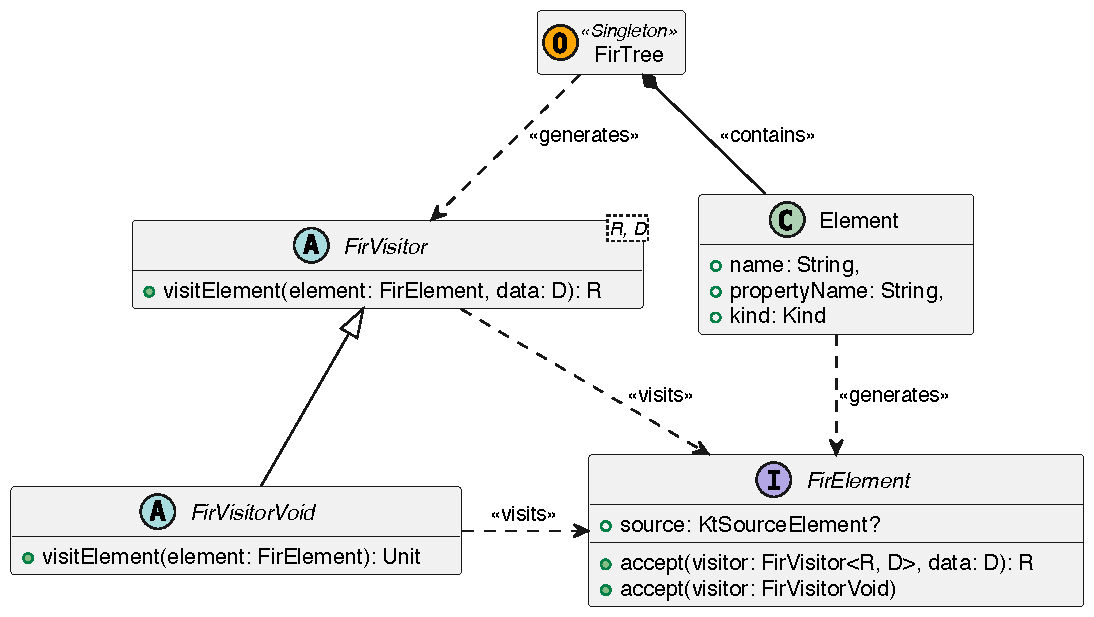
\includegraphics[width=.7\linewidth]{figures/fir-visitors.pdf}
  \caption{Summarized class diagram of the visitors inside the Kotlin 
  compiler}
  \label{fig:fir-visitors-class-diagram}
\end{figure}

\subsection{Pattern 3: unnecessary Yielding usage}

Having introduced the visitor pattern, we can now see it in practice having 
to deal with the next pattern, whose implementation in the checkers exploited
\ac{FIR} visitors. This pattern regard the \emph{unnecessary usage of the} 
\lstinline{yielding} \emph{contexts} in the Collektive DSL. 
%
The \lstinline{yielding} context is a specific feature inside the Collektive
\ac{DSL}, briefly introduced in \cref{sec:collektive-dsl}, that allows the
developer to call a construct of the \ac{DSL}, like \lstinline{exchange} for
instance, returning a value different from the result of the construct. To use
this feature, instead of using the actual construct, the variant with the
\lstinline{-ing} suffix is used, like \lstinline{exchanging} in this case, and
these variants are called called \textbf{yielding operations}. 
%
Essentially, a \lstinline{YieldingContext<Initial, Return>} is used inside
yielding operations to act on an \lstinline{Initial} value --- that can, for
example, be exchanged with neighbors --- but \textbf{return a different value of
type} \lstinline{Return} to the caller, without having to return the same value
as for the normal version.

In \cref{lst:p3-yielding-example} we can see an example of the usage of this
yielding context, taken from the Collektive documentation. 

\lstinputlisting[
  float, 
  language=Kotlin, 
  label={lst:p3-yielding-example},
  caption={Example of usage of the yielding context in the Collektive DSL, 
  taken from the Collektive documentation}
]{listings/P3YieldingExample.kt}

In the example provided, the \lstinline{exchanging} construct will still perform
like the normal \lstinline{exchange} construct, which sends the results from the
evaluation of the passed function to other devices and returns an object of type
\lstinline{Field<Int, Int>}, but the entire operation will return another object
of type \lstinline{Field<Int, String>}, resulted from the \lstinline{map} call
inside the yielding action.

As it may have been guessed, the usage of this feature can be redundant: nothing
prevents the developer from using this construct and return the same value as the
one been computed and sent to the other devices by the construct, resulting in a 
completely useless \lstinline{yielding} that could be safely substituted with the
normal version of the construct. 
%
An example of this Pattern is shown in \cref{lst:p3-example}.

\lstinputlisting[
  float, 
  language=Kotlin, 
  label={lst:p3-example},
  caption={Example of Pattern 3 detection in code, with an unecessary usage of a
  yielding context, this time with the \lstinline{sharing} construct}
]{listings/P3Example.kt}

\subsubsection{Formal description}

Given a Collektive construct that accepts a \lstinline{YieldingContext} as
parameter (e.g., \lstinline{exchanging}, \lstinline{evolving}, etc.), the
pattern is satisfied when the expression returned inside the anonymous function
passed as parameter to the \lstinline{yielding} call is \emph{equivalent} to the
one used as its \emph{receiver}, therefore resulting in a redundant usage of the
yielding context. 

\subsubsection{Design and Implementation}

As previously introduced, this Pattern's checker will be based on the Visitor
pattern. The checker can simply perform an initial check on the function name to
intercept a Collektive construct that accepts a \lstinline{YieldingContext},
based on a set of predefined, fully-qualified names. 
%
Once one of these constructs is found, the checker will delegate the inspection
of the anonymous function to the implemented visitor, that will traverse the
small part of the \ac{FIR} tree that is contained within the construct's
parameters (i.e., the anonymous function passed as parameter to the construct)
%
Finally, the visitor will return a boolean value used to report the successful
or unsuccessful detection of the pattern.

The implementation of the checker can be seen in \cref{lst:p3-checker}. The core
part is, of course, the visitor method call
\lstinline{containsUnnecessaryYielding}, whose implementation will be briefly
discussed in the following.

\lstinputlisting[
  float, 
  language=Kotlin, 
  label={lst:p3-checker},
  caption={Implementation of the Pattern 3 checker: \lstinline{UnnecessaryYielding}}
]{listings/P3Checker.kt}

\subsubsection{Visitor implementation}

To check if a function call corresponding to a construct with a yielding context
matches the pattern, we need to inspect the anonymous function that is passed as
parameter. When the visitor encounters a function call to the
\lstinline{yielding} operation, it will simply save the \textbf{explicit
receiver} of the call and then visit the anonymous function that is passed as
parameter to \lstinline{yielding}.
%
When visiting a \emph{return expression} of the anonymous function
passed to the yielding construct, the visitor will check if the expression is
\emph{equivalent} to the saved receiver of the yielding construct.
%
If so, the visitor will return \lstinline{true}, meaning that the pattern is
detected, otherwise it will return \lstinline{false}. 

A behavior like this can be easily implemented using the
\lstinline{FirVisitorVoid} class: the \cref{lst:p3-visitor} summarizes the visitor's
implementation.

\lstinputlisting[
  float, 
  language=Kotlin, 
  label={lst:p3-visitor},
  caption={Implementation of the Pattern 3 Visitor}
]{listings/P3Visitor.kt}

The function \lstinline{isStructurallyEquivalentTo} is a utility function that
uses Kotlin \emph{expression rendering} to check if two expressions are 
equivalent. For brevity purposes, its implementation is omitted.
%
The function \lstinline{containsUnnecessaryYielding} is also omitted, but its
implementation is a simple as calling the visiting methods and return a boolean
variable set during the exploration.

It appears quite clear how a visitor approach to this task is very effective and
limited in complexity compared to using the \ac{FIR} API on the elements
directly. However, this still represents a very simple case, often solved by
common static analysis checks for programming languages in similar situations
(e.g., same expression on both sides of an assignment). Let's see how to 
approach more complex cases with the visitor pattern.

\subsection{Pattern 4: unnecessary construct usage}

In order to prove the effectiveness of the visitor pattern in more complex cases,
we will now present a more complex pattern that can be detected using this
approach. This pattern regards the \emph{unnecessary usage of constructs} in the
Collektive DSL.

Kotlin compiler won't, by default, warn the developer when an anonymous function
that can have one or more parameters is created without using them in the body 
(and maybe passed to another function as a parameter). For example in the code
shown in the following snippet:

\begin{lstlisting}[language=Kotlin]
listOf(1, 2, 3).map { 5 }
\end{lstlisting}

The anonymous function passed to the \lstinline{map} function is not using the
\lstinline{it} parameter and, in general, this cannot always be interpreted as
an error because, depending on the function, the parameter might not be needed.
%
Some Collektive constructs, however, are designed to work with the parameters of
these anonymous functions, and the absence of these parameters could be a sign
of misinterpretation of the construct's behavior and intended usage as well as 
an unnecessary network exchange that results in a waste of resources.

Not all constructs behave in the same way: for example, the
\lstinline{neighboring} and \lstinline{neighboringViaExchange} constructs are
different from the rest. Since these two functions evaluate expressions in
neighbors devices, if the expression to evaluate is provided as an anonymous
function, this does not accept parameters. In this case, the construct usage is
considered unnecessary if the anonymous function has an \emph{empty return} ---
i.e., a return of type \lstinline{Unit}. 
%
An example of both the cases is shown in \cref{lst:p4-example}.

\lstinputlisting[
  float, 
  language=Kotlin, 
  label={lst:p4-example},
  caption={Examples of Pattern 4 detection in code, with both the cases described}
]{listings/P4Example.kt}

\subsubsection{Formal description}

Given a Collektive construct that accepts an anonymous function as parameter,
the pattern is satisfied when the body of the anonymous function does not use the
parameters that its signature accepts \emph{or} when the body of the anonymous
function returns \lstinline{Unit} in absence of accepted parameters (i.e., the
\lstinline{neighboring} and \lstinline{neighboringViaExchange} constructs).

\subsubsection{Design and Implementation}

Similarly to the previous pattern, the checker will be implemented with a very
simple logic, exploiting more complex visitors to inspect the pattern matching.
In this case, the checker will simply check if a function call is one of the 
Collektive constructs to check. If so, it will delegate the inspection on one
of two visitors, whether the construct is one of the constructs that accept
anonymous functions with parameters or not.

The implementation is summarized in \cref{lst:p4-checker}. As we can see, the
two visitors are \lstinline{EmptyReturnVisitor} and
\lstinline{ConstructCallVisitor}. The former is quite simple to implement (and,
therefore, will be explained without code): it behaves like a default
visitor, but when visiting a \lstinline{FirReturnExpression} element, it checks
if the return type is \lstinline{FirUnitExpression}. If so, the pattern is
detected.

\lstinputlisting[
  float, 
  language=Kotlin, 
  label={lst:p4-checker},
  caption={Implementation of the Pattern 4 checker: 
  \lstinline{UnnecessaryUseOfConstructs}}
]{listings/P4Checker.kt}

The second visitor is more complex: when checking for usages of parameters, we
\textbf{cannot simply check the return expression of the anonymous function} and
see if it uses the parameters, because the parameters can be used in other
expressions to create \textbf{dependent symbols} --- i.e., symbols that depend
on and can be used instead of the parameters in the return expression.
%
To solve this problem in a more simple way, the visitor will \textbf{not} check
if the dependent symbols are used in the return expression, therefore
implementing a \emph{symbol marking} system, but instead it will simply consider
the pattern as detected once it sees at least one usage of the parameter inside
the anonymous function body.  

The implementation of the \lstinline{ConstructCallVisitor} is shown in
\cref{lst:p4-visitor}. The variable \lstinline{found} will be set to
\lstinline{true} when the visitor encounters a usage of all parameters, meaning
that the pattern is detected when \lstinline{!found}. This is the result
obtained by the visitor calling its utility method shown in the checker. 

\lstinputlisting[
  float, 
  language=Kotlin, 
  label={lst:p4-visitor},
  caption={Implementation of the Pattern 4 Visitor}
]{listings/P4Visitor.kt}

The visitor approach works very well also in this case: the code is sufficiently
readable and simple to understand. Even though the logic is more complex
compared to the previous cases, however, we are not yet dealing with patterns
that require to visit \textbf{more distant elements} in the \ac{FIR} tree, for
example \emph{visiting the function declaration of a function call} or
\emph{linking the usage of a symbol to its declaration}. 

Despite these considerations, it is already possible to see some drawbacks of
this approach: the code is already becoming less declarative, having to use
\emph{flags} to keep track of the state of the visitor for example preventing
some visit methods to be called in contexts we don't want them to be called
(e.g., in the visitor just presented, the case of nested anonymous functions). 

\section{4th approach: mixed approach}

In order to avoid the possible pitfalls of the visitor pattern that would make
this approach less scalable to the increasing complexity of the pattern, we can
use a mixed approach that combines the visitor pattern with the simple API we
previously introduced. The main advantage over other static analysis tools, in
fact, is that the tree we are visiting is already enriched with a lot of
information that the visitor can use inside its visit methods to perform checks,
therefore avoiding the need to visit the tree in a more complex way.
%
We can also create utility functions that call other visitors to extract
information useful for the checker or another visitor. Making this structure 
modular and extensible is key for the success of this approach.

\subsection{Pattern 5: complex aggregate operations in loops} \label{sec:p5}

The case of aggregate operations in loops was already treated in \cref{sec:p2},
but the pattern was not completely covered, (intentionally) presenting the
pattern's description in a non-complete way. In particular, a special usage
case was omitted, here called the case of \textbf{delegated functions}. 
%
In this case, the construct is not directly called inside the loop, but it is
\emph{delegated to another function that is called inside the loop}. This
function is not necessarily a nested function, as in the case already seen in
\cref{sec:p2}, but it can be a function that is defined elsewhere in the code:
from now on, this will be called the \emph{delegated function} or simply the
\emph{delegate}. In order to contain aggregate calls, the delegate must have a
parameter of type \lstinline{Aggregate} to use as a receiver for the aggregate
constructs (if, instead the delegate would have an explicit receiver of type
\lstinline{Aggregate}, in fact, the pattern would be trivially detected by the
Pattern 2 checker, as the delegate would appear as an aggregate construct
itself).
%
Just like before, this case adds surprising complexity to the pattern even with
just a small additional constraint to its definition. The plethora of possible
cases that can be captured in the code by this pattern is quite large, and some
examples are shown in \cref{lst:p5-example}. Seeing the second example should
give an idea of how many possible code variations are related to this pattern,
and why this additional constraint has been treated as a separated pattern with
respect to Pattern 2.

\lstinputlisting[
  float, 
  language=Kotlin, 
  label={lst:p5-example},
  caption={Examples of Pattern 5 detection in code, with the case of delegated
  functions}
]{listings/P5Example.kt}

\subsubsection{Formal description}

Given a looping construct (like the ones already seen for Pattern 2) and a
declared function, here called \emph{delegate}, whose parameters list contains
one of type \lstinline{Aggregate} and whose body contains an aggregate construct
call, the pattern is satisfied when \emph{delegate} is called inside the loop or
in a chain of other function calls that ends with a call inside the loop, and
neither \emph{delegate} nor the functions in the chain contain an
\lstinline{alignedOn} operation wrapping one of the calls.

\subsubsection{Design and Implementation}

To implement this pattern, a new condition will be added to the checker seen in
\cref{lst:p2-checker} that will handle the case of delegated functions. The new
condition will perform the same checks as the previous one (i.e., is inside a
looping construct and it is not aligned) but instead of checking if the function
call being examined is an aggregate one, it will check if one of its parameters
is of type \lstinline{Aggregate}. To do this, a new utility function is
implemented: \lstinline{hasAggregateParameter}, shown in \cref{lst:p5-utility}.
%
\begin{lstlisting}[
  float, 
  language=Kotlin,
  label={lst:p5-utility},
  caption={Utility function to check if a function call has an aggregate parameter}
]
fun FirFunctionCall.hasAggregateArgument(): Boolean =
  getArgumentsTypes()?.any {
      it.classId == ClassId.topLevel(AGGREGATE_CLASS_FQ_NAME.toFqNameUnsafe())
  } ?: false 
\end{lstlisting}
%
This uses the \lstinline{getArgumentsTypes} and \lstinline{toFqNameUnsafe}
extension methods that have been implemented for the job (and are omitted for
brevity). 

Once this condition is satisfied, the visitor will be called to
inspect the delegate function and check if it contains an aggregate construct
call or a call to another function that contains an aggregate construct call
(possibly in a chain of calls). \textbf{Note:} we cannot use the code already
implemented for Pattern 2 for checking the presence of the \lstinline{alignedOn}
operation, since its call could be in a different function that is called inside
the delegate and that is not directly one of the \emph{containing elements} of
the aggregate construct call. For this reason, the visitor will be used also for
this purpose.

To implement this visitor, we need a way to visit the function declaration
associated with the function call that is being visited. Thanks to Kotlin API,
this can be done like seen in \cref{lst:p5-declaration}.
%
\begin{lstlisting}[
  float, 
  language=Kotlin,
  label={lst:p5-declaration},
  caption={Simple utility function to get the declaration of a function call}
]
@OptIn(SymbolInternals::class)
fun FirFunctionCall.getDeclaration(): FirSimpleFunction? =
  calleeReference.toResolvedFunctionSymbol()?.fir as? FirSimpleFunction
\end{lstlisting}
%
The \lstinline{@OptIn} is necessary in order to access the \lstinline{fir}
field. Once this is done, we need to visit the function declaration and check
its body for the pattern presence. In addition, however, we also need to be
careful to detect \emph{nested function declarations}, and for this reason 
a \lstinline{functionCounter} variable is used to keep track of the nesting
level of the function declarations. 
%
The other elements we need to visit are the function calls contained in the body
of the function. The only functions we are interested in are of two types:

\begin{enumerate}
  \item \textbf{Aggregate function calls}: function calls that require alignment
  or \lstinline{alignedOn} operations;
  \item \textbf{Function calls with aggregate parameter (i.e., delegates)}: this 
  functions could recursively contain dangerous function calls, so are targeted 
  by other checks
\end{enumerate}

In the first case, we check if the function call is an alignment operation, and if
so we accept its anonymous function parameter with the visitor keeping track that 
we are inside an alignment (i.e., so other aggregate operations are considered safe
within it). If the aggregate function is not an alignment operation and we are not
\emph{inside an alignment or nested function}, the pattern is detected.

In the second case we simply instantiate another visitor and recursively visit the
function call in question, checking if the pattern is detected in the delegate.

The implementation just explained is summarized in \cref{lst:p5-visitor}.
Although the code is still short like for the other visitors, in this case we
need to take \emph{multiple visiting calls} of the same method and even
\emph{recursive visiting} with an another visitor into consideration.

\subsubsection{Considerations on this pattern}

Unfortunately, some corner cases are not still captured by this checker and
visitor: the main reason is that some corner cases that involve the usage of
local variables from nested functions, similar to the second case shown in
\cref{lst:p5-example} without alignment present, are difficult to capture with
the current approach. Since it is not a common usage case, it was decided to
leave it for future works. It is a good opportunity, however, to reason about
how what it has been developed so far presents, from time to time, some
branching conditions in the code or some particular programming ``tricks'' that
appear as fragile or poorly maintainable code. 
%
This aspect is related to the ``defensive'' approach for developing these static
checkers: one could think that detecting the pattern is the core of the
implementation but, in reality, one of the most important aspects is
\textbf{being careful not to introduce false positives} to the static analysis.
%
This is logical, since the cases we are trying to capture are actually a very
small subset of the possible programs using the Collektive DSL (and Kotlin in
general). This is also the reason why adding more complex checks like the one
just described has to be taken with much caution, and it is of main importance
to add \textbf{more tests for cases where the pattern is not detected} than for
cases where it is detected.
%
The approach taken for testing this important factor will be discussed in the
next chapter: for now, we will move to the final pattern, the one that was
considered the most complex to detect, where multiple types of visitors were
used together to inspect the code.

\lstinputlisting[
  float, 
  language=Kotlin, 
  label={lst:p5-visitor},
  caption={Implementation of the Pattern 5 Visitor}
]{listings/P5Visitor.kt}
 
\subsection{Pattern 6: improper Evolve construct usage}

The last pattern presented in this chapter involves three of the constructs of the 
Collektive DSL that we have seen: \lstinline{evolve}, \lstinline{neighboring}
and \lstinline{share} (and their variants with the yielding context).
%
The \lstinline{evolve} construct is used to evolve the value of a device,
iteratively updating it with the results of a function that is passed as a
parameter. The \lstinline{neighboring} construct is used to evaluate an
expression in neighbors, constructing a \lstinline{Field} object mapping the
neighbors to the results of the evaluation. The \lstinline{share} construct is
used to compute a \emph{space-time} evolution of the field, computing an
expression over time and sharing it with the neighbors. Since the
\lstinline{evolve} construct too can be used to evolve a field over time, its
combination with the \lstinline{neighboring} construct can behave exactly like a
\lstinline{share}, since the second one can be used to map the \emph{space}
aspect. 
%
This is not always true, of course, but using the \lstinline{evolve} construct
could easily lead to this inefficient usage of the DSL constructs,  especially
if the developer is not aware of constructs like \lstinline{share}.

This pattern consists specifically in this type of usage of the \lstinline{evolve}
construct. Since the anonymous function passed to it as a parameter must return
a value of the same type of the one gave to it as \emph{initial} one, a user could
first use the \lstinline{neighboring} construct to evaluate the expression in 
neighbors and then perform a \emph{field reduction} operation --- e.g., finding the
max value in the field --- and return that as the result of the anonymous function.
%
Different is the case in which the \lstinline{neighboring} construct is used to 
evaluate a different expression that \textbf{does not depend on the value updated
by evolve} and therefore will share a value independently of the one evolved.

These examples of usage and related version with the \lstinline{share} construct 
substituted are shown in \cref{lst:p6-example}.

\lstinputlisting[
  float, 
  language=Kotlin, 
  label={lst:p6-example},
  caption={Example of Pattern 6 detection in code}
]{listings/P6Example.kt}

\subsubsection{Formal description}

Given an \lstinline{evolve} construct that is passed a function that contains a
\lstinline{neighboring} construct, the pattern is satisfied when the expression
evaluated by the \lstinline{neighboring} construct depends on the value of
evolve, and it is used to compute the value returned by the anonymous function
passed to the \lstinline{evolve} construct.

\subsubsection{Design and Implementation}

The mixed approach previously introduced will be fully exploited to implement
this checker. In order to \emph{trace the dependencies} between the expressions
that relate to the evolved value --- i.e., the parameter inside the
\lstinline{evolve} anonymous function --- we need a system to \emph{mark
expressions} that use this value and then maintain a list of symbols that are
dependent on the evolved value. 
%
When these symbols are used in other expressions, we then mark theses as
dependent on the evolved value as well and so on. When we encounter a
\lstinline{neighboring} construct, we can immediately know if the expression
evaluated by it depends on the evolved value, and if not the check can
immediately end.
%
If the expression depends on the evolved value, we must save the evaluated
expression and continue the visit until the end of the anonymous function with
the return expression. Obtained the return expression, we must first extract the 
receiver of the \lstinline{yielding} construct if the aggregate construct used 
is a variant with the yielding context, or simply the expression itself if not. 
%
This extra step is necessary for the variants of the construct because the 
value returned by the \lstinline{yielding} is not really relevant to the pattern
detection, since it will be returned as it is either way. 
%
Finally, we must check if the expression is \textbf{not} equivalent to the one
evaluated by the \lstinline{neighboring} construct, and if so the pattern is
detected. 

Since the workflow is not straightforward, a diagram of the process is shown in
\cref{fig:p6-workflow}.
%
\begin{figure}
  \centering
  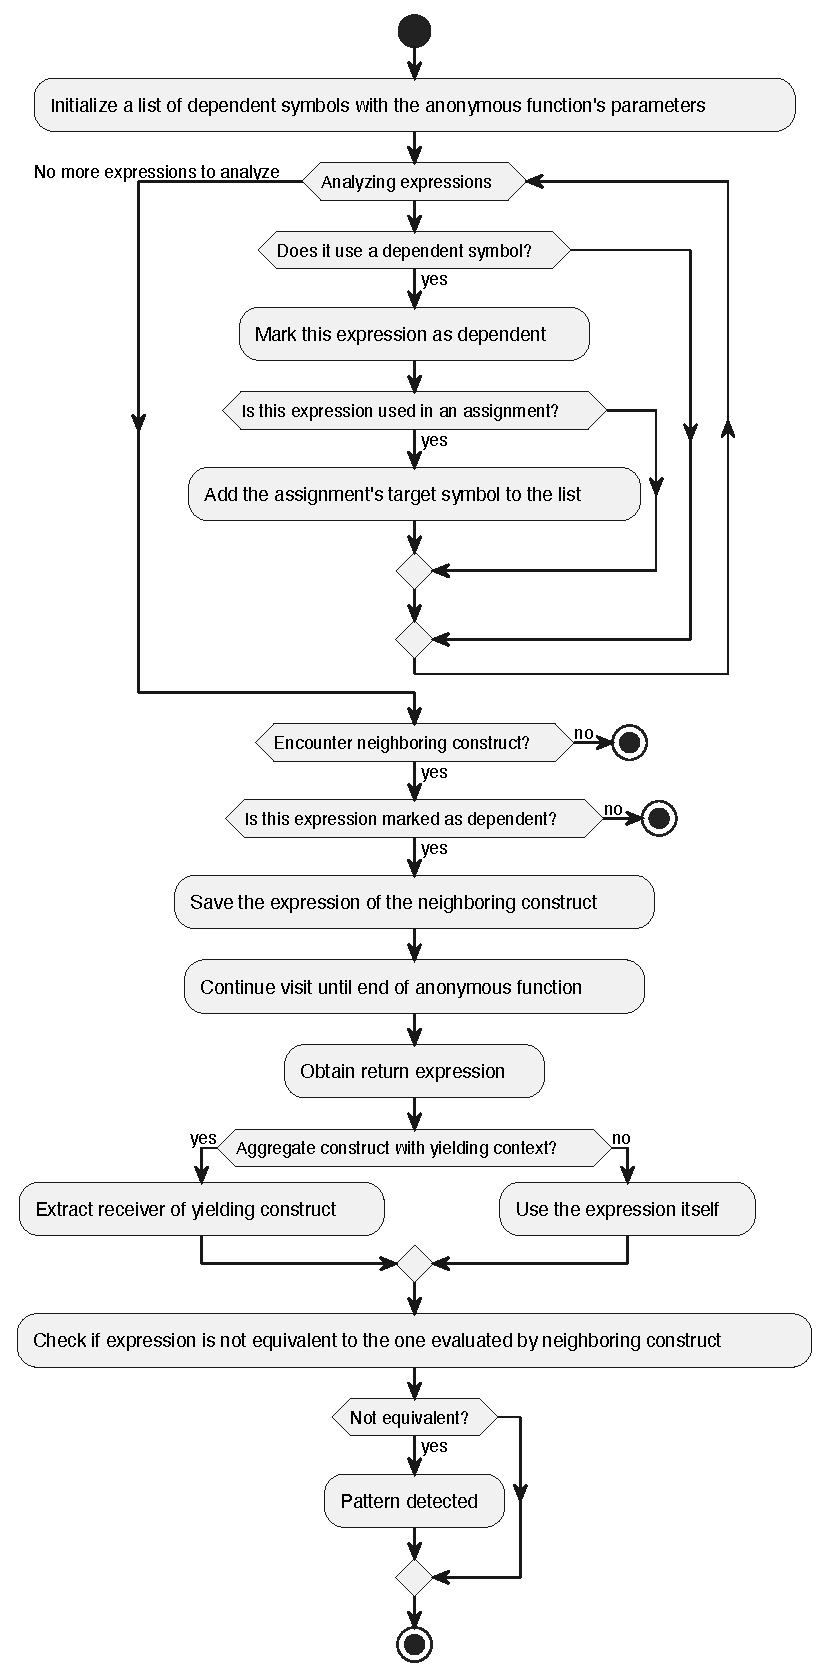
\includegraphics[width=.6\linewidth]{figures/p6-workflow.pdf}
  \caption{Summarized workflow of the Pattern 6 detection}
  \label{fig:p6-workflow}
\end{figure}
%
As for the previous patterns implemented using visitors, the implementation of
the checker is quite simple and therefore omitted. The visitor, however, will
need a specific section to be treated in detail. 

\subsubsection{Visitor implementation}

The first element the visitor is going to visit is, again, a function call
corresponding to a Collektive \ac{DSL} construct, specifically the
\lstinline{evolve} construct and its variant. In this case, the visitor will
simply access the construct and look inside its parameters --- i.e., the 
anonymous function. 
%
When this is done, the visitor will switch to the visit
method of the anonymous function, where first it will check if this function
is a \textbf{top nesting level} and not a nested function (for the first 
visit it obviously is) and will access the \textbf{function parameters} and
add them to a list of \emph{dependent symbols} kept by the visitor.
%
In \cref{lst:p6-visit-anonymous} this procedure is shown.
%
\begin{lstlisting}[
  float, 
  language=Kotlin,
  label={lst:p6-visit-anonymous},
  caption={Visitor method to visit an anonymous function}
] 
override fun visitAnonymousFunctionExpression(anonymousFunctionExpression: FirAnonymousFunctionExpression) {
  if (nestingLevel == 0) {
      val anonymousFunction = anonymousFunctionExpression.anonymousFunction
      val parameters = anonymousFunction.valueParameters
      parametersDeclarations = parameters.map { it.symbol }
  }
  nestingLevel++
  super.visitAnonymousFunctionExpression(anonymousFunctionExpression)
  nestingLevel--
}
\end{lstlisting}
%
The visitor will then visit the body of the anonymous function. Every time the
visitor encounters a \lstinline{FirResolvedNameReference}, corresponding to a
symbol usage, it will check if the symbol is contained in the list of dependent
symbols. If so, the visitor will set a variable \lstinline{markExpression} to
\lstinline{true}, meaning that the expression is dependent on the evolved value.
%
In this way, when the visitor encounters a property (i.e., local variable), it
will check if the expression is marked as dependent and, if so, it will add the
property to the list of dependent symbols. This is shown in
\cref{lst:p6-visit-property}.
%
\begin{lstlisting}[
  float, 
  language=Kotlin,
  label={lst:p6-visit-property},
  caption={Visitor methods to implement a symbol and expression marking system}
]
override fun visitResolvedNamedReference(ref: FirResolvedNamedReference) {
    if (ref.resolvedSymbol in parametersDeclarations ||
        ref.resolvedSymbol in tracedDependentSymbols
    ) {
        markExpression = true
    }
}

override fun visitProperty(property: FirProperty) {
    if (markExpression) {
        tracedDependentSymbols += property.symbol // add the symbol to the list
        markExpression = false
    }
}
\end{lstlisting}
%
These methods take care of the tracing of the dependent symbols, now it is
necessary to approach the core of the visitor: the \lstinline{neighboring} and
return expressions. 

The first one can be inspected when the visitor encounters a function call, and
then check for the fully-qualified name of the construct. In that case, we can
extract the expression used as parameter to the construct and perform the
necessary checks. The \lstinline{neighboring} construct can be used essentially
in two ways:
\begin{enumerate}
  \item \textbf{Direct expression}: for example a numerical expression like a
  sum between two numbers;
  \item \textbf{Computation}: for example an anonymous function, in that case
  the field returned by the construct has the computation as a result, in the 
  form of a field of functions.
\end{enumerate}

In the first case, we can simply obtain the first argument of the construct,
verify if the expression is \emph{marked} when visiting it and, if so, set a
variable that \textbf{contains the expression for later}. In the second case, we
must visit the anonymous function and obtain the return expression, and then
perform the same operations. To do this, a utility function is implemented that
\textbf{extracts the return expression of an anonymous function using another
visitor}. The implementation is shown in \cref{lst:p6-support-visitor}. In this
case, we create a visitor on the fly and visit the anonymous function, returning
the expression found. This is an example of how composing visitors with the
\ac{FIR} API can work.

\lstinputlisting[
  float, 
  language=Kotlin, 
  label={lst:p6-support-visitor},
  caption={First support visitor to extract the return expression of an anonymous 
  function}
]{listings/P6SupportVisitor1.kt}

Once we saved the expression evaluated by the \lstinline{neighboring} construct,
a comparison with the return expression of the anonymous function is needed to
complete the detection of the pattern. When the visitor encounters the return
expression, it must first check if the nesting level is correct and if the
expression of the \lstinline{neighboring} construct if present. If not, the
pattern is skipped. Finally, to compare the return expression with the
expression of the construct using the \lstinline{isStructurallyEquivalentTo}
utility function previously introduced, we must handle a last special case: the
yielding context. 

In the case of the yielding context, the expression returned by the
\lstinline{yielding} construct is not relevant to the pattern detection, and so
its \textbf{receiver} must be used instead. To get the receiver, another support 
visitor is implemented, shown in \cref{lst:p6-support-visitor2}.

\lstinputlisting[
  float, 
  language=Kotlin, 
  label={lst:p6-support-visitor2},
  caption={Second support visitor to extract the receiver of a yielding construct}
]{listings/P6SupportVisitor2.kt}

The visitor is used in the visit method of the return expression, performing the
final check on the equivalence of the expressions. If the expressions are not
equivalent, the pattern is detected. The implementation of this last visit method 
is shown in \cref{lst:p6-visit-return}.

\begin{lstlisting}[
  float, 
  language=Kotlin,
  label={lst:p6-visit-return},
  caption={Visitor method to visit the return expression}
]
override fun visitReturnExpression(returnExpression: FirReturnExpression) {
  super.visitReturnExpression(returnExpression)
  if (neighboringExpression != null && nestingLevel == 1) {
    val expressionToCheck = neighboringExpression as FirExpression
    if (constructNameFQName == EVOLVING_FUNCTION_FQ_NAME) {
      // case with yielding context
      val yieldingReceiver =
        with(YieldingReceiverVisitor()) {
          returnExpression.getYieldingReceiver()
        } ?: return
      isReplaceable = !yieldingReceiver.isStructurallyEquivalentTo(expressionToCheck)
    } else {
      isReplaceable = !returnExpression.result.isStructurallyEquivalentTo(expressionToCheck)
    }
    return
  }
}
\end{lstlisting}

With this, all the patterns that were considered for the Collektive DSL static
analysis have been implemented. As discussed in this chapter, many approaches
were taken and in some cases mixed together to achieve the desired results.
Since the presented patterns were not shown in their order of implementation, it
is possible to see some areas of improvement, especially in the first
ones implemented using the visitor pattern. 
%
Other considerations about this development process as well as other possible 
ways to implement the checkers will be matter of discussion in the conclusions 
of \cref{chap:conclusion}. First, the testing strategy that was adopted during 
these checkers' implementation will be presented.

%----------------------------------------------------------------------------------------
\chapter{Evaluation and Testing}
\label{chap:evaluation}
%----------------------------------------------------------------------------------------

When developing tools that need to inspect and modify source code, where
developers have freedom to write code in many ways and leveraging the full power of the 
used programming language, a solid and comprehensive testing strategy is crucial to 
ensure that the tool is working as expected and that it is able to capture all the
cases that it is supposed to capture.
%
If static analysis tools can be tedious to develop, due to the need to cover a
plethora of possible cases, often with a unified meta-level approach, testing
static analysis tools must be even more comprehensive and flexible than
development, trying not to fall into verbosity and repetition.

In this chapter we will present the testing strategy that was adopted to test the 
Collektive frontend plugin, starting from the initial approaches and moving into the 
development of an \emph{ad-hoc} testing framework named \emph{Subjekt}.

\section{Initial testing approaches}

The first approach taken was the most trivial: the tests were written using
\textbf{static Kotlin sources} as resource files, loading them in the test
suites written using the Kotlin test framework \textbf{Kotest}. The first
problem that arose regarded the \emph{compilation process and the check for
resulting diagnostics}. To test the checkers, in fact, the code must be compiled
programmatically also providing the plugin to the compiler, and then collect all
the produced messages and compare them with the expected ones.
%
Fortunately, a library already exists for this purpose: \textbf{Kotlin Compile
Testing} by Thilo Schuchort (tschuchortdev on GitHub)\footnote{The actual
library that was used is a fork of the original one, maintained by Zac Sweers
(ZacSweers on GitHub). The switch to the fork was necessary due to some issues
encountered during the building process of the project with Kotlin 2.0 which,
at the time of writing, is still not supported by the original library. More
information is available here:
\url{https://github.com/tschuchortdev/kotlin-compile-testing/issues/411}}.
This library provides a simple way to create objects that represent Kotlin source
files by passing a string source code, and then compile them giving a list of
compiler plugins or annotation processors that should be used during the
compilation process. All of this is done \emph{inheriting the class path} of
where the compilation process is running, so the Collektive plugin can be added
without any problem also adding the corresponding library. Finally, the
diagnostics produced are contained inside the
\lstinline{KotlinCompilation.Result} object as a single string that can be
easily split and filtered to get the relevant messages and compare them with the
expected ones.

With this library, it is now possible to write tests simply by reading the
resource files that contain the source code that should result or not in a
pattern being detected. These testing cases should be the same that were
extracted from the codebase during the development of the checkers. An example
of a test suite using this method can be seen in \cref{lst:initial-test-suite}.
%
\lstinputlisting[
  float, 
  language=Kotlin, 
  label={lst:initial-test-suite},
  caption={One of the first developed test for the Pattern 2 checker. It uses
  static resource files to load the source code to be compiled and checked}
]{listings/TestingExample1.kt}
%
As we can see, the testing process is quite simple and straightforward:
\lstinline{TestAggregateInLoop.kt} is a source file contained in the resource
folder and contains a simple source code with an aggregate construct used inside
a loop, which is the case that should be detected by the checker for Pattern 2.

It appears quite clear however, how this approach soon proves to be un-scalable
and especially very repetitive, as for the same pattern to be tested there are
many possible source codes in which the checker might have to operate (and
therefore cases to be tested) and where the difference with the previous ones
is, in most cases, a line or two of code. 
%
Following this method, the test suite would have needed many static files, each
very similar to some others, and the Kotest spec would have been very verbose,
even trying to minimize the repeated parts through the use of Kotest utility
functions like \lstinline{forAll}.

\section{Avoiding repetitions through template files}

One of the first solutions to the problem of repetition when dealing with
textual files very similar to each other is to use \textbf{template files}. The
approach is quite simple: for each pattern to test, collapse all the testing
cases that are similar to each other into a single file containing placeholders
for the parts that change. 

\subsection{Initial template system}

The initial template system consisted of simple Kotlin files containing the
source code to be compiled with placeholders like the ones used in classical
string formatting --- i.e., \lstinline{%s}. An example is shown in 
\cref{lst:template-file}. 
%
\lstinputlisting[
  language=Kotlin, 
  label={lst:template-file},
  caption={A example of the templates created for testing multiple cases at 
  once}
]{listings/TestingTemplateFile.kt}
%
Then, instead of compiling the string obtained from the resource file directly,
replace the placeholders cycling through a list of possible, hard-coded
configurations in the test suite and for each perform the correct check on the
diagnostics produced.
%
In addition, we extracted a small utility in order to make the process of
reading resources, compiling and comparing messages more concise and readable
using Kotlin infix methods.
The result looks similar to the one shown in \cref{lst:template-test-suite}.
Only a relevant part of the test suite is shown, the rest is omitted for
brevity.

\lstinputlisting[
  language=Kotlin, 
  label={lst:template-test-suite},
  caption={Part of the test for Pattern 2 revised using template files}
]{listings/TestingExample2.kt}

\subsection{Templates flexibility and limitations}

Even though this approach gained some flexibility and reduced repetitions on the
template files side, it still requires a lot of boilerplate code to be written
between each test case. Another step is necessary to make the testing process
even more concise: integrating the created utility with a string interpolation
mechanism that allows configurable parts without repeated and obscure code for
formatting. 
%
This allows to write templates that are more clear and readable, because instead
of writing placeholders with \lstinline{%s} we can write variables with names 
like \lstinline{%(nameOfTemplateVariable)} and then pass a configurable map 
through the test code that will replace these variables with the correct values.
All of these utilities, contained in the singleton object \lstinline{CompileUtils},
permit writing tests like the ones shown in \cref{lst:template-revised-suite}.
%
\lstinputlisting[
  float, 
  language=Kotlin, 
  label={lst:template-revised-suite},
  caption={\Cref{lst:template-test-suite} revised using the new utilities}
]{listings/TestingExample3.kt}
%
Variables also have default values, making the tests more concise and easier to
write. It is easy to see how the test not only gained in readability, but it is
much more scalable and can be used to test many more cases adding only a few
lines of code. 

The obtained result, however, is still far from optimal: the testing code still
depends too much on the structure of the template files, exploiting hard-coded
names of variables inside the template files and in the test suite. The problem
still relies on the fact that \textbf{the testing resource doesn't encapsulate
the possible values of its variable}, making it more flexible indeed but also
less maintainable and more error-prone. 
%
Without using a system more similar to a \emph{template engine}, it would be
difficult to build the testing process without occurring in scale issues,
especially for more complex patterns discussed in \cref{chap:contribution} where
the number of possible cases to test is much higher than the ones presented in
the examples. Even in that case, however, the testing process would have to
interact with the templates in order to determine values of its variable parts,
also for \textbf{identifying the expected outcomes} of the resulting source
code's compilation. In other words, there still would be too much coupling
between the testing code and resource files.

\section{Code generation: a small DSL leveraging Kotlin Poet}

A possible approach to solve the problem of coupling between the testing code
and the resource files is \textbf{code generation done directly inside tests}.
Instead of using external files, a developer could create an appropriate
configuration in the tests to capture a multitude of cases, declaratively 
specifying how the source code should be structured and therefore knowing at
prior what the expected diagnostics should be.
%
It is quite clear that the task is not an easy one, since generating multiple 
source codes in a declarative way using the same programming language as the
target one is not trivial. Thankfully, an already existing and well-known 
library can be used for the generation: \textbf{Kotlin Poet} by Square Inc.

Kotlin Poet is a library with a Java and Kotlin API to generate Kotlin sources.
Its main use cases are generating code for annotation processors or interacting
with metadata files, and it is inspired by another library by the same authors,
Java Poet. 
%
The library is quite powerful and allows generating code in a declarative way,
using a fluent API to create complex structures with few lines of code. One
way to use it is through a \emph{builder} pattern, where methods are chained to
create the desired structure. This particular way of generating code can reveal
itself as very useful for our purpose, since it can be manipulated to build a 
\ac{DSL} that facilitates some operations for the developer.

\subsection{General structure and usage}

To make the generation of code more concise and readable, a \ac{DSL} has been
created using \textbf{extension methods to the Kotlin Poet builders}.
Encapsulating the generation of common code and frequent and repeated operations
inside these methods, allows for a completely customizable output with a few
lines of code, using constructs tailored for our testing cases. 
%
Take the extensions shown in \cref{lst:poet-extensions} for example: in this
case we create utilities to build programs with blocks and specific wrapping
functions, like the \lstinline{alignedOn} seen in \cref{sec:p2} during the
explanation of Pattern 2. 
%
\lstinputlisting[
  float, 
  language=Kotlin, 
  label={lst:poet-extensions},
  caption={Example of Kotlin Poet extensions used to generate code}
]{listings/KotlinPoetMethods.kt}
%
This way, the developer can pass other extension methods --- e.g., parameter
\lstinline{content} visible in \cref{lst:poet-extensions} --- to these
\ac{DSL}-like keywords to highly customize the final output, therefore 
maintaining Kotlin Poet benefits but also making it more directed to 
our needs. 

Finally, it is possible to rewrite the tests, using no external resource file
and reusing the same pieces of code that do not change across the several
checks. A small snippet of how this small \ac{DSL} can be used in tests is shown
in \cref{lst:poet-test-suite}.

\lstinputlisting[
  language=Kotlin, 
  label={lst:poet-test-suite},
  caption={Example of a test suite using the Kotlin Poet extensions}
]{listings/TestingExample4.kt}

Imagining various checks to be done for Pattern 2 --- the one the examples of
this chapter are based on --- this approach greatly reduces the amount of
boilerplate code, intervening only inside the function containing the call
to the aggregate construct and the loop construct, and then customizing it 
with other parts, like the \lstinline{alignedOn} construct that wraps the 
tested function call. 
%
At last, the expected diagnostics are formulated starting from the case that is
being generated and tested and compared with the one produced by the compilation
thanks to the Kotlin Compile Testing library already cited. 
%
This last operation is encapsulated inside the small utility library already
implemented for the previous testing approaches, adding also the customized
function to the source code: this summarizes what is done at line 18 of
\cref{lst:poet-test-suite}.

\subsection{Considerations}

The approach of code generation seems to be the most flexible and scalable 
solution to the problem at hand: even though it wasn't considered worth the 
effort to integrate a system like this in the first stages of the development,
patterns examined further in the thesis showed how many possible cases 
required a proper a more complete testing strategy without falling into
verbosity and repetition (e.g., Pattern 5 and Pattern 6).
%
Nevertheless, more complex test cases, where more than just a couple of lines of
code change, still require considerable effort to create Kotlin sources subject
to compilation. With the small \ac{DSL} created, the approach just described
tends to become less readable and harder to interpret, to the point that in
cases where there isn't enough common code, it becomes easier to write the code
directly as a single string.

It seems that the problem still regards static resource files in a sense: even
though common parts of the code are reused and customized with the \ac{DSL}, the
``variability'' of general-purpose languages like Kotlin makes it difficult to
reduce possible Kotlin sources to something like templates or customizable parts
of code.
%
For these reasons, this small \ac{DSL} was not integrated into the Collektive
project, but it was used as a starting point to develop a more complete and
flexible testing framework that could be used to test the Collektive frontend
plugin in a more comprehensive way. 

\section{Custom testing framework: Subjekt}

\emph{Subjekt} is a tool for generating textual results starting from a
configuration in YAML or JSON format. It can be used to generate multiple
results from permutations of parameters of the configuration, easily creating
many variations of the same output.
%
This tool started as a simple utility to generate multiple Kotlin sources from a
starting configuration and then integrate them inside Collektive test projects.
Later in the development process, it was decided to expand its capabilities to
directly generate test cases for the Collektive plugin from inside the test
suites, adding only the configurations as resources.

Subjekt is a small Kotlin multiplatform library available on \emph{Maven
Central}, \emph{npmjs} and GitHub packages repositories. In this section we will
present the main benefits of using a tool like this for testing static analysis
projects like the Collektive frontend plugin.

\subsection{Main ideas behind the framework}

The main inspiration behind Subjekt is the testing strategy used by the
\emph{Scala}
compiler\footnote{\url{https://github.com/scala/scala3/tree/main/tests}} (on
a smaller scale of course).
% 
Essentially, the core idea is to set up a suite of \emph{test cases} having
expected positive or negative outcomes. In the Scala compiler, source code and
expected outcomes are separated into \emph{.scala} and \emph{.check} files,
respectively. 
%
Subjekt follows a similar approach, but linking together source and expected
outputs. The developer can write a configuration file in YAML or JSON format
reflecting a \textbf{suite} of test \textbf{subjects} that are related to 
a similar pattern to be tested. 
%
As for Scala, every testing case has a unique identifier, and in the case of
Subjekt can be extracted from the result of the generation to refer to a 
specific test case in the suite.

\subsection{Core structure of Subjekt}

In Subjekt, each configuration file defines a \textbf{Suite}, composed by a list
of \textbf{Subjects}. Each Subject is essentially a map with string keys and
values, where the latter contain \textbf{Expressions}: strings with expressions
are called \textbf{Resolvables}. 
%
The expressions are strings that are parsed to generate a multitude of results:
\emph{Subjekt} will extract these results and produce a set of outputs
considering all the permutations of the expressions contained in the subjects.
Special delimiters \lstinline|${{| and \lstinline|}}| are used in order to
extract expressions from strings, inspired by the GitHub actions expressions
syntax\footnote{
\url{https://docs.github.com/en/actions/writing-workflows/choosing-what-your-workflow-does/evaluate-expressions-in-workflows-and-actions}
}.
%
The diagram in \cref{fig:subjekt-structure} shows the general class diagram of 
the library.

\begin{figure}
  \centering
  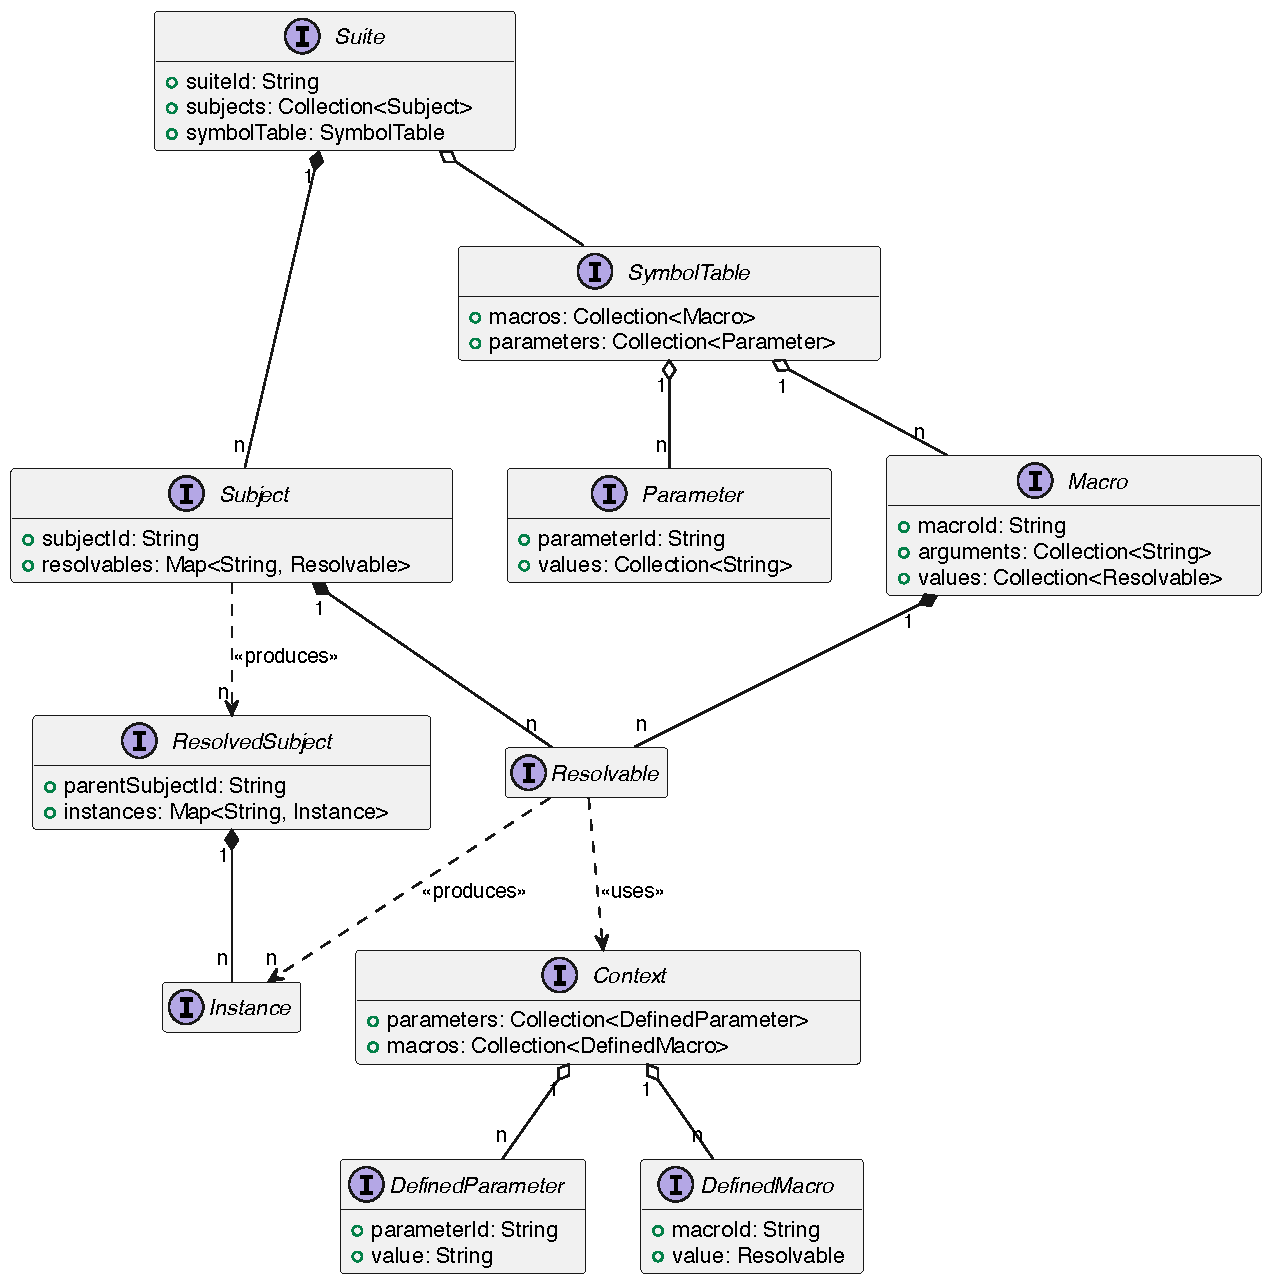
\includegraphics[width=.8\linewidth]{figures/subjekt-structure.pdf}
  \caption{Top-level class diagram of the Subjekt library}
  \label{fig:subjekt-structure}
\end{figure}

The main entities that produce permutations are \textbf{Parameters} and
\textbf{Macros}. Both of them can have multiple values to substitute in the
expressions where they are used, but the difference is that the former's values
do not contain other expressions, while the latter's ones are actually other
Resolvables and can accept arguments to substitute in their expressions ---
i.e., a kind of function that returns multiple values --- leading to an
exponential growth of the number of results (for example when other Parameters
are passed to the Macro, making Subjekt produce permutations of the passed
Parameter's values and the Macro's ones).
%
When a Resolvable needs to be resolved, the Subjekt library will determine all
the possible \textbf{Contexts} that can be generated from the Parameters and
Macros. Each Context will contain one ``fixed'' value for each of them --- i.e.,
\textbf{DefinedParameter} and \textbf{DefinedMacro} --- and will therefore 
correspond to one of the total permutations.
%
The Resolvable will finally produce one \textbf{Instance} for each of the
Contexts.

The final result are the \textbf{ResolvedSubjects}. Each of these is
essentially one of the generated outputs, and can be used to contain one of the
source codes to be compiled and the expected diagnostics to be checked.
%
The output is actually a set of these object to avoid testing the same case
multiple times in case of collisions due to the permutations of the expressions.

\subsection{Final usage inside tests}

As previously introduced, Subjekt can be configured using YAML or JSON format.
To use it inside Collektive in order to produce testing cases, a resource file
will be created for each pattern to be tested, containing the entirety of cases
for that pattern. In order to test them, we will create a Kotest specification
for each Subjekt configuration, that gets loaded using the Subjekt library and
then executed comparing the diagnostics produced by the compilation with the
expected ones.

Ultimately, the Kotlin Compile Testing library was abandoned in favor of a
custom solution that uses a utility singleton named
\lstinline{CollektiveK2JVMCompiler} that automatically compiles a list of source
files returning the diagnostics produced via a \lstinline{MessageCollector} and
using the Collektive compiler plugin. 

In \cref{lst:subjekt-suite} a small example of a simple Subjekt configuration
used for the tests of Pattern 2 is shown. In this configuration
\lstinline{loop}, \lstinline{prettify} and \lstinline{AGGREGATE} are
respectively two Macros and one Parameter that are omitted for brevity. The
first one wraps the argument with several types of iteration constructs, for
example a \lstinline{for} loop or a \lstinline{map} method call on a list. The
second is a Macro exposed by Subjekt in all its configurations and that is used
to concatenate any number of arguments into a camel case, special
characters-free formatted string. The last one is a Parameter that contains a
list of aggregate construct to be tested in the source code (e.g.,
\lstinline{neighboring}).

\lstinputlisting[
  float, 
  language=Yaml,
  label={lst:subjekt-suite},
  caption={Example of a Subjekt configuration file used for Pattern 2 testing.}
]{listings/SubjektExample.yaml}

The configuration file is then loaded inside the test suite, and the subjects
are resolved and executed. The expected diagnostics are then compared with the
ones produced by the compilation, and the test is considered successful if they
match. In \cref{lst:subjekt-test-suite} a small snippet of the test suite using
Subjekt is shown.

\lstinputlisting[
  language=Kotlin,
  label={lst:subjekt-test-suite},
  caption={Example of a test suite using Subjekt}
]{listings/TestingExample5.kt}

As we can see, the test suite is quite concise and readable, and can be easily
expanded to test more cases by adding more configurations to the resource file.
Moreover, inside the Kotest specification the developer does not have to worry
about the details of the source being compiled or the diagnostics produced and,
with an appropriate implementation of the check, if a test fails it is easy to
immediately see the source code that caused the failure and the expected
diagnostics that were not produced, leading to an efficient test-driven
development cycle.

Subjekt is still a small library that can be expanded and improved in order to
make the creation of tests even more automatized and with less repetitions, but
its approach represents a possible solution to the problem of testing static
analysis tools that was faced during the development of the Collektive frontend
plugin for this thesis.

%----------------------------------------------------------------------------------------
\chapter{Conclusions}
\label{chap:conclusion}
%----------------------------------------------------------------------------------------

In this chapter we will present the conclusions of the work done during the
thesis, starting from the main contributions and the results obtained, and then
moving to the discussion of the limitations and possible future works that can
be done to improve the Collektive frontend plugin as well as static analysis 
tools via compiler plugins in general.

\section{Opportunities of Compiler plugins}

Compiler plugins represent a very powerful tool for developers that want to
customize a specific ``environment'' within a framework written in a general
purpose language. If brought to a sufficient degree of integration, they can
embrace the full power of \emph{internal} \acp{DSL}, breaking some remaining
barriers between the domain and the host language. If added to an automatically
integrated static analysis tool like a frontend compiler plugin, it can also
help developers to avoid common obstacles to the adoption of new tools and 
``languages'' in their projects, speeding up the learning process of the new
constructs and the spreadness of new paradigms.

In this thesis, the development of the Collektive frontend plugin showed an
example of how this can be approached in a real use case, and how the
interaction with the compiler can happen in a seamless way, potentially leading
to libraries made specifically to build Kotlin compiler plugins enhancing the
already existing, still limited and experimental, K2 frontend API.
%
Through the development of the plugin, it was interesting to see how spotting
new patterns to be caught with static analysis immediately corresponded to their
implementation directly in the same tool used to enable the target \ac{DSL}.
This helped understand just how much bringing static analysis towards the tool
that is being analyzed can be beneficial, since it allowed to immediately spot
bad usages inside already existing code, therefore leading to the formulation of
new patterns to be detected and building a virtuos cycle of improvement of the
whole framework. Moreover, such a development could exploit this opportunity to
delegate bad usages of the \ac{DSL} to the compiler, making the developer's life
easier and the codebase more robust, without having to rely on ``programming
tricks'' or forced limitations of the language to avoid bad usages.
%
Finally, using a unified approach to the static analysis tool development, in 
this case the frontend compiler plugin, can greatly facilitates the inclusion 
of such a tool in the development environment, making it interact with the 
\ac{IDE} and build system automatically and without the need of additional
\ac{IDE} plugin or other types of necessary integrations, often developed by
third parties and not always up-to-date with the latest versions of the
frameworks.

In order to show a solid development process of such a plugin, covering the
full spectrum of the cycle, more effort was put into building an effective
testing strategy that could be used to test also a bigger number of patterns
even more complex than the ones presented in this thesis. This led to the 
exploration of different testing approaches, each one with its own pros and
cons, and finally to a more scalable and flexible method, accompanied by
the small testing framework Subjekt, developed exactly for this purpose.

\section{Approaching meta-level analysis}

In this thesis, multiple techniques have been employed to build checkers capable
of identifying increasingly complex patterns, ultimately relying on the widely
used \emph{visitor pattern}. This choice was necessary to align with Kotlin's
\ac{FIR} API, which, while offering extensive capabilities, remains closely
tied to the compiler's internal structures. 
%
However, this strong coupling highlights a broader challenge: the lack of a
higher-level abstraction for static analysis within compiler plugins. As
demonstrated, performing pattern-based checks requires directly traversing and
manipulating the tree, making the implementation more intricate and less
maintainable. This underlines the importance of elevating compiler plugins to a
\textbf{meta-level}, where analysis can be expressed through a specialized
meta-language rather than being deeply intertwined with compiler internals. 
%
Such an approach, similar to what other static analysis tools already provide,
enhances at least three aspects of the analysis tool:
\begin{itemize}
  \item \textbf{expressiveness}: meta-level languages already exists in order
  to capture complex patterns and relationships between code constructs, and
  can be used to express the analysis in a more concise and readable way;
  \item \textbf{maintainability}: by decoupling the analysis logic from the
  compiler-level representation, it becomes easier to adapt to language 
  evolution and ensure more scalable and reliable checks;
  \item \textbf{modularity}: the analysis can be split into smaller, more
  manageable components, focusing on specific aspects of the pattern 
  being checked. 
\end{itemize}

Thus, while the \ac{FIR} API enables powerful static analysis, the need for a
higher-level abstraction remains crucial to making these techniques more
accessible, flexible, and efficient in the long term.

\section{Future works}

At the moment of writing, the Kotlin API that enables static analysis in
frontend plugins like the one seen in this thesis is still highly experimental,
therefore subject to changes and improvements. Developing a meta-level language
tool for this API could be a possible future work, but it would require a more
stable and mature version of the API to be effective.
%
Despite this, working on a unified language similar to the one used in other
static analysis tools could be a good starting point, maybe based on
\emph{tree-based pattern matching} techniques or other more advanced methods.
This could allow compiler plugins to become easier to use and more accessible
to developers, leveraging the full power of this type of system. 
%
Other than that, allowing compiler plugins to use configuration files already
used by other tools like \emph{Detekt} would strenghten the idea of the unified
approach even more, making the compiler plugin approach an interesting choice 
as a standards for static analysis tools on the Kotlin platform.

Another possible future work could involve the testing method, expanding the
automatized approach taken with the Subjekt framework to be more inclusive and
flexible, allowing the developer to test more complex patterns with less effort,
maybe even in a way that is tied to the meta-level language used for the checks.
%
Finally, the development of the Collektive frontend plugin could be expanded to
include more patterns and more complex checks, maybe arose after a more in-depth
usage of the \ac{DSL} in a real project, in order to make the plugin more
complete and effective in spotting bad usages of the available constructs.

The Kotlin ecosystem is one of the most vibrant and fast-growing, thanks to its
flexibility and the wide range of platforms it can target. Compiler plugins are
a powerful tool that can be used to enhance the development process and the
quality of the code produced, bringing paradigms that struggle to be adopted
into the mainstream. 
%
Empowering developers to use these tools more seamlessly across this vast
landscape of platforms and projects could unlock their true hidden potential,
turning them into a powerful asset rather than a niche solution.



%----------------------------------------------------------------------------------------
% BIBLIOGRAPHY
%----------------------------------------------------------------------------------------

\backmatter

\nocite{*} % Remove this as soon as you have the first citation

\bibliographystyle{alpha}
\bibliography{bibliography}

\begin{acknowledgements} % this is optional
Optional. Max 1 page.
\end{acknowledgements}

\end{document}
